\documentclass[10pt, a4paper, english]{article}\usepackage[]{graphicx}\usepackage[dvipsnames]{xcolor}
% maxwidth is the original width if it is less than linewidth
% otherwise use linewidth (to make sure the graphics do not exceed the margin)
\makeatletter
\def\maxwidth{ %
  \ifdim\Gin@nat@width>\linewidth
    \linewidth
  \else
    \Gin@nat@width
  \fi
}
\makeatother

\definecolor{fgcolor}{rgb}{0.345, 0.345, 0.345}
\newcommand{\hlnum}[1]{\textcolor[rgb]{0.686,0.059,0.569}{#1}}%
\newcommand{\hlstr}[1]{\textcolor[rgb]{0.192,0.494,0.8}{#1}}%
\newcommand{\hlcom}[1]{\textcolor[rgb]{0.678,0.584,0.686}{\textit{#1}}}%
\newcommand{\hlopt}[1]{\textcolor[rgb]{0,0,0}{#1}}%
\newcommand{\hlstd}[1]{\textcolor[rgb]{0.345,0.345,0.345}{#1}}%
\newcommand{\hlkwa}[1]{\textcolor[rgb]{0.161,0.373,0.58}{\textbf{#1}}}%
\newcommand{\hlkwb}[1]{\textcolor[rgb]{0.69,0.353,0.396}{#1}}%
\newcommand{\hlkwc}[1]{\textcolor[rgb]{0.333,0.667,0.333}{#1}}%
\newcommand{\hlkwd}[1]{\textcolor[rgb]{0.737,0.353,0.396}{\textbf{#1}}}%
\let\hlipl\hlkwb

\usepackage{framed}
\makeatletter
\newenvironment{kframe}{%
 \def\at@end@of@kframe{}%
 \ifinner\ifhmode%
  \def\at@end@of@kframe{\end{minipage}}%
  \begin{minipage}{\columnwidth}%
 \fi\fi%
 \def\FrameCommand##1{\hskip\@totalleftmargin \hskip-\fboxsep
 \colorbox{shadecolor}{##1}\hskip-\fboxsep
     % There is no \\@totalrightmargin, so:
     \hskip-\linewidth \hskip-\@totalleftmargin \hskip\columnwidth}%
 \MakeFramed {\advance\hsize-\width
   \@totalleftmargin\z@ \linewidth\hsize
   \@setminipage}}%
 {\par\unskip\endMakeFramed%
 \at@end@of@kframe}
\makeatother

\definecolor{shadecolor}{rgb}{.97, .97, .97}
\definecolor{messagecolor}{rgb}{0, 0, 0}
\definecolor{warningcolor}{rgb}{1, 0, 1}
\definecolor{errorcolor}{rgb}{1, 0, 0}
\newenvironment{knitrout}{}{} % an empty environment to be redefined in TeX

\usepackage{alltt}
%typesetting
\usepackage[margin = 1in]{geometry} % margins
\usepackage[T1]{fontenc} % font encoding
\usepackage{babel} %enables typesetting for multiple languages
\usepackage{parskip} %new lines
\usepackage{graphicx} 
\usepackage{float}
\floatplacement{figure}{H} %when printing tables, include  table.position="H"
\usepackage{bm}
\usepackage{amsmath}

\usepackage[dvipsnames]{xcolor} % more colors

\usepackage[colorlinks]{hyperref}


 %clickable table of contents from hyperref
\hypersetup{
    colorlinks,
    citecolor=black,
    filecolor=black,
    linkcolor=black,
    urlcolor=black
}

\usepackage[colorinlistoftodos]{todonotes}


\title{Machine Learning 2ST129 26605 HT2023
 Assignment 4}
\author{Anonymous Student}
\date{\today}
\IfFileExists{upquote.sty}{\usepackage{upquote}}{}
\begin{document}
\maketitle
\newpage
\tableofcontents
\newpage

\section*{General Information}
\begin{itemize}
\item Time used for reading: 2 hours: 
\item Time used for basic assignment: 18 hours 
\item Time used for extra assignment: 6 hours 
\item Good with lab: It was good that you had had to tune different hyper parameters and think about what they are doing.
\item Things improve with lab: Maybe more explanation about how to plot images and how to code works. I do not really know what I am doing, I just copy paste the code given for some part and use other packages for another part. 
\end{itemize}





\section{Task 1}
\begin{knitrout}
\definecolor{shadecolor}{rgb}{0.969, 0.969, 0.969}\color{fgcolor}\begin{kframe}
\begin{alltt}
\hlcom{#Libraries}
 \hlkwd{library}\hlstd{(tidyverse)}
 \hlkwd{library}\hlstd{(xtable)}
 \hlkwd{library}\hlstd{(tensorflow)}
 \hlkwd{library}\hlstd{(keras)}
\end{alltt}
\end{kframe}
\end{knitrout}

\begin{knitrout}
\definecolor{shadecolor}{rgb}{0.969, 0.969, 0.969}\color{fgcolor}\begin{kframe}
\begin{alltt}
\hlstd{mnist} \hlkwb{<-} \hlkwd{dataset_mnist}\hlstd{()}
\hlstd{mnist}\hlopt{$}\hlstd{train}\hlopt{$}\hlstd{x} \hlkwb{<-} \hlstd{mnist}\hlopt{$}\hlstd{train}\hlopt{$}\hlstd{x}\hlopt{/}\hlnum{255}
\hlstd{mnist}\hlopt{$}\hlstd{test}\hlopt{$}\hlstd{x} \hlkwb{<-} \hlstd{mnist}\hlopt{$}\hlstd{test}\hlopt{$}\hlstd{x}\hlopt{/}\hlnum{255}
\hlstd{x_train} \hlkwb{<-} \hlstd{mnist}\hlopt{$}\hlstd{train}\hlopt{$}\hlstd{x}
\hlstd{x_test} \hlkwb{<-} \hlstd{mnist}\hlopt{$}\hlstd{train}\hlopt{$}\hlstd{x}
\hlcom{#Since the reponse variablbe y is an vector with integer values with 10 classes,}
\hlcom{# we need to one-hot encode them into binary class matrices}
\hlcom{#}
\hlstd{y_train} \hlkwb{<-} \hlkwd{to_categorical}\hlstd{(mnist}\hlopt{$}\hlstd{train}\hlopt{$}\hlstd{y,} \hlkwc{num_classes} \hlstd{=} \hlnum{10}\hlstd{)}
\hlstd{y_test} \hlkwb{<-} \hlkwd{to_categorical}\hlstd{(mnist}\hlopt{$}\hlstd{test}\hlopt{$}\hlstd{y,} \hlkwc{num_classes} \hlstd{=} \hlnum{10}\hlstd{)}
\end{alltt}
\end{kframe}
\end{knitrout}
% We can now refer to it as Figure \ref{fig:my_plot}.
\subsection{1.1}
First we visualize the digits.
\begin{knitrout}
\definecolor{shadecolor}{rgb}{0.969, 0.969, 0.969}\color{fgcolor}\begin{kframe}
\begin{alltt}
\hlcom{#' function to iterate through the different idx and plot the images}
\hlstd{plot_images} \hlkwb{<-} \hlkwa{function}\hlstd{(}\hlkwc{image_array}\hlstd{,} \hlkwc{y}\hlstd{,} \hlkwc{idx}\hlstd{,} \hlkwc{pixel_dim} \hlstd{=} \hlnum{28}\hlstd{,} \hlkwc{ncol} \hlstd{=} \hlnum{3}\hlstd{,} \hlkwc{pred}\hlstd{=}\hlnum{FALSE}\hlstd{) \{}
  \hlkwd{par}\hlstd{(}\hlkwc{mfrow} \hlstd{=}\hlkwd{c}\hlstd{(}\hlnum{1}\hlstd{,}\hlnum{3}\hlstd{))}

  \hlkwa{for} \hlstd{(i} \hlkwa{in} \hlstd{idx) \{}
    \hlstd{im} \hlkwb{<-} \hlstd{image_array[i,,]}
    \hlstd{im} \hlkwb{<-} \hlkwd{t}\hlstd{(}\hlkwd{apply}\hlstd{(im,} \hlnum{2}\hlstd{, rev))}
    \hlkwa{if} \hlstd{(}\hlkwd{isFALSE}\hlstd{(pred))\{}
      \hlstd{main} \hlkwb{<-} \hlkwd{paste}\hlstd{(y[i])}
    \hlstd{\}} \hlkwa{else}\hlstd{\{}
\hlstd{main} \hlkwb{<-} \hlkwd{paste}\hlstd{(}\hlstr{"Actual: "}\hlstd{,} \hlkwd{paste0}\hlstd{(y[i],}\hlstr{","}\hlstd{),} \hlstr{"Predicted:"}\hlstd{, pred[i])}
    \hlstd{\}}
  \hlkwd{image}\hlstd{(}\hlnum{1}\hlopt{:}\hlstd{pixel_dim,} \hlnum{1}\hlopt{:}\hlstd{pixel_dim, im,} \hlkwc{col} \hlstd{=} \hlkwd{gray}\hlstd{((}\hlnum{0}\hlopt{:}\hlnum{255}\hlstd{)}\hlopt{/}\hlnum{255}\hlstd{),}
            \hlkwc{xlab} \hlstd{=} \hlstr{""}\hlstd{,} \hlkwc{ylab} \hlstd{=} \hlstr{""}\hlstd{,} \hlkwc{xaxt} \hlstd{=} \hlstr{'n'}\hlstd{,} \hlkwc{yaxt} \hlstd{=} \hlstr{'n'}\hlstd{,}
        \hlkwc{main} \hlstd{= main)}
  \hlstd{\}}

  \hlkwd{par}\hlstd{(}\hlkwc{mfrow} \hlstd{=} \hlkwd{c}\hlstd{(}\hlnum{1}\hlstd{,} \hlnum{1}\hlstd{))}
\hlstd{\}}
\end{alltt}
\end{kframe}
\end{knitrout}

\begin{knitrout}
\definecolor{shadecolor}{rgb}{0.969, 0.969, 0.969}\color{fgcolor}\begin{kframe}
\begin{alltt}
\hlkwd{plot_images}\hlstd{(}\hlkwc{image_array} \hlstd{= x_train,} \hlkwc{y} \hlstd{= mnist}\hlopt{$}\hlstd{train}\hlopt{$}\hlstd{y,} \hlkwc{idx} \hlstd{=} \hlkwd{c}\hlstd{(}\hlnum{1}\hlopt{:}\hlnum{3}\hlstd{))}
\end{alltt}
\end{kframe}\begin{figure}
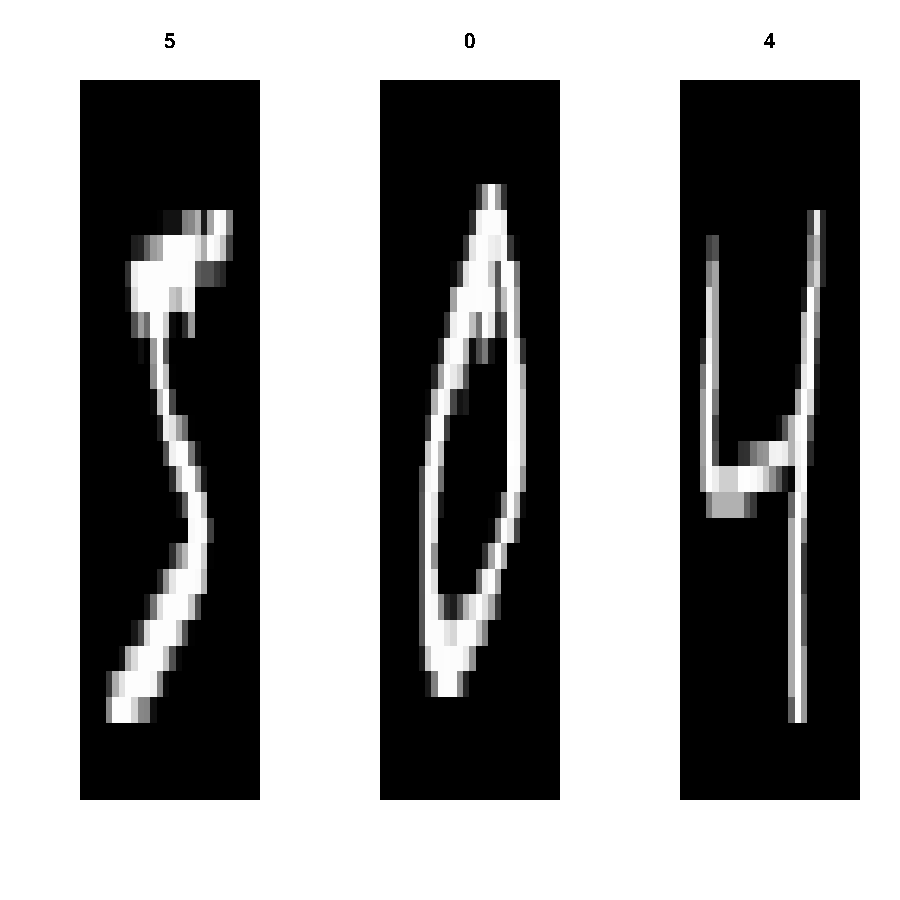
\includegraphics[width=\maxwidth]{figure/unnamed-chunk-4-1} \caption[Visualization of first 3 digits in mnist data set]{Visualization of first 3 digits in mnist data set}\label{fig:unnamed-chunk-4}
\end{figure}

\end{knitrout}

\subsection{1.2 Convulutional neural network}
\begin{knitrout}
\definecolor{shadecolor}{rgb}{0.969, 0.969, 0.969}\color{fgcolor}\begin{kframe}
\begin{alltt}
\hlstd{model1} \hlkwb{<-} \hlkwd{keras_model_sequential}\hlstd{()} \hlopt
  \hlkwd{layer_conv_2d}\hlstd{(}\hlkwc{filters} \hlstd{=} \hlnum{32}\hlstd{,} \hlkwc{kernel_size} \hlstd{=} \hlkwd{c}\hlstd{(}\hlnum{3}\hlstd{,} \hlnum{3}\hlstd{),} \hlkwc{activation} \hlstd{=} \hlstr{'relu'}\hlstd{,}
                \hlkwc{input_shape} \hlstd{=} \hlkwd{c}\hlstd{(}\hlnum{28}\hlstd{,} \hlnum{28}\hlstd{,} \hlnum{1}\hlstd{))} \hlopt
  \hlkwd{layer_max_pooling_2d}\hlstd{(}\hlkwc{pool_size} \hlstd{=} \hlkwd{c}\hlstd{(}\hlnum{2}\hlstd{,} \hlnum{2}\hlstd{))} \hlopt
  \hlkwd{layer_conv_2d}\hlstd{(}\hlkwc{filters} \hlstd{=} \hlnum{32}\hlstd{,} \hlkwc{kernel_size} \hlstd{=} \hlkwd{c}\hlstd{(}\hlnum{3}\hlstd{,} \hlnum{3}\hlstd{),} \hlkwc{activation} \hlstd{=} \hlstr{'relu'}\hlstd{)} \hlopt
  \hlkwd{layer_flatten}\hlstd{()} \hlopt
  \hlkwd{layer_dense}\hlstd{(}\hlkwc{units} \hlstd{=} \hlnum{64}\hlstd{,} \hlkwc{activation} \hlstd{=} \hlstr{'relu'}\hlstd{)} \hlopt
  \hlkwd{layer_dense}\hlstd{(}\hlkwc{units} \hlstd{=} \hlnum{10}\hlstd{,} \hlkwc{activation} \hlstd{=} \hlstr{'softmax'}\hlstd{)}


\hlkwd{summary}\hlstd{(model1)}
\end{alltt}
\begin{verbatim}
Model: "sequential"
________________________________________________________________________________
 Layer (type)                       Output Shape                    Param #     
================================================================================
 conv2d_1 (Conv2D)                  (None, 26, 26, 32)              320         
 max_pooling2d (MaxPooling2D)       (None, 13, 13, 32)              0           
 conv2d (Conv2D)                    (None, 11, 11, 32)              9248        
 flatten (Flatten)                  (None, 3872)                    0           
 dense_1 (Dense)                    (None, 64)                      247872      
 dense (Dense)                      (None, 10)                      650         
================================================================================
Total params: 258090 (1008.16 KB)
Trainable params: 258090 (1008.16 KB)
Non-trainable params: 0 (0.00 Byte)
________________________________________________________________________________
\end{verbatim}
\end{kframe}
\end{knitrout}



\subsection{1.3}
The reason there are 320 parameters in the first layer is due to the filter and kernel size. We have 32 filters  where the filter size or kernel\_size is $ 3\times 3$. Hence the number of parameters becomes $(3 \times 3 + 1) \times 32 = 10 \times 32 = 320$  where the additional 1 is the bias (and hence 1 per filter) and the rest are the kernel weights. 

\subsection{1.4}
\begin{knitrout}
\definecolor{shadecolor}{rgb}{0.969, 0.969, 0.969}\color{fgcolor}\begin{kframe}
\begin{alltt}
\hlstd{model1} \hlopt \hlkwd{compile}\hlstd{(}
  \hlkwc{optimizer} \hlstd{=} \hlstr{'RMSprop'}\hlstd{,}\hlcom{# RMSPROP instead of adam}
  \hlkwc{loss} \hlstd{=} \hlstr{'categorical_crossentropy'}\hlstd{,}
  \hlkwc{metrics} \hlstd{=} \hlkwd{c}\hlstd{(}\hlstr{'accuracy'}\hlstd{)}
\hlstd{)}

\hlstd{history} \hlkwb{<-} \hlstd{model1} \hlopt \hlkwd{fit}\hlstd{(}
  \hlstd{x_train, y_train,}
  \hlkwc{epochs} \hlstd{=} \hlnum{10}\hlstd{,}\hlkwc{batch_size} \hlstd{=} \hlnum{128}\hlstd{,}
  \hlkwc{validation_split} \hlstd{=} \hlnum{0.2}\hlstd{,}
  \hlkwc{callbacks} \hlstd{=} \hlkwd{list}\hlstd{(}\hlkwd{callback_early_stopping}\hlstd{(}\hlkwc{patience} \hlstd{=} \hlnum{5}\hlstd{,} \hlkwc{monitor}\hlstd{=}\hlstr{"val_loss"}\hlstd{))}
\hlstd{)}
\end{alltt}
\end{kframe}
\end{knitrout}

Here it stopped early. The bets results are from epoch 4. The loss and accuracy metrics are given by:

\begin{knitrout}
\definecolor{shadecolor}{rgb}{0.969, 0.969, 0.969}\color{fgcolor}\begin{kframe}
\begin{alltt}
375/375 [==============================] - 11s 29ms/step 
- loss: 0.0390 - accuracy: 0.9876 - val_loss: 0.0482 - val_accuracy: 0.9854
\end{alltt}
\end{kframe}
\end{knitrout}

And the plot over the history of the accuracy and loss per epoch:
\begin{knitrout}
\definecolor{shadecolor}{rgb}{0.969, 0.969, 0.969}\color{fgcolor}\begin{kframe}
\begin{alltt}
\hlstd{knitr}\hlopt{::}\hlkwd{include_graphics}\hlstd{(}\hlstr{"model1.png"}\hlstd{)}
\end{alltt}
\end{kframe}
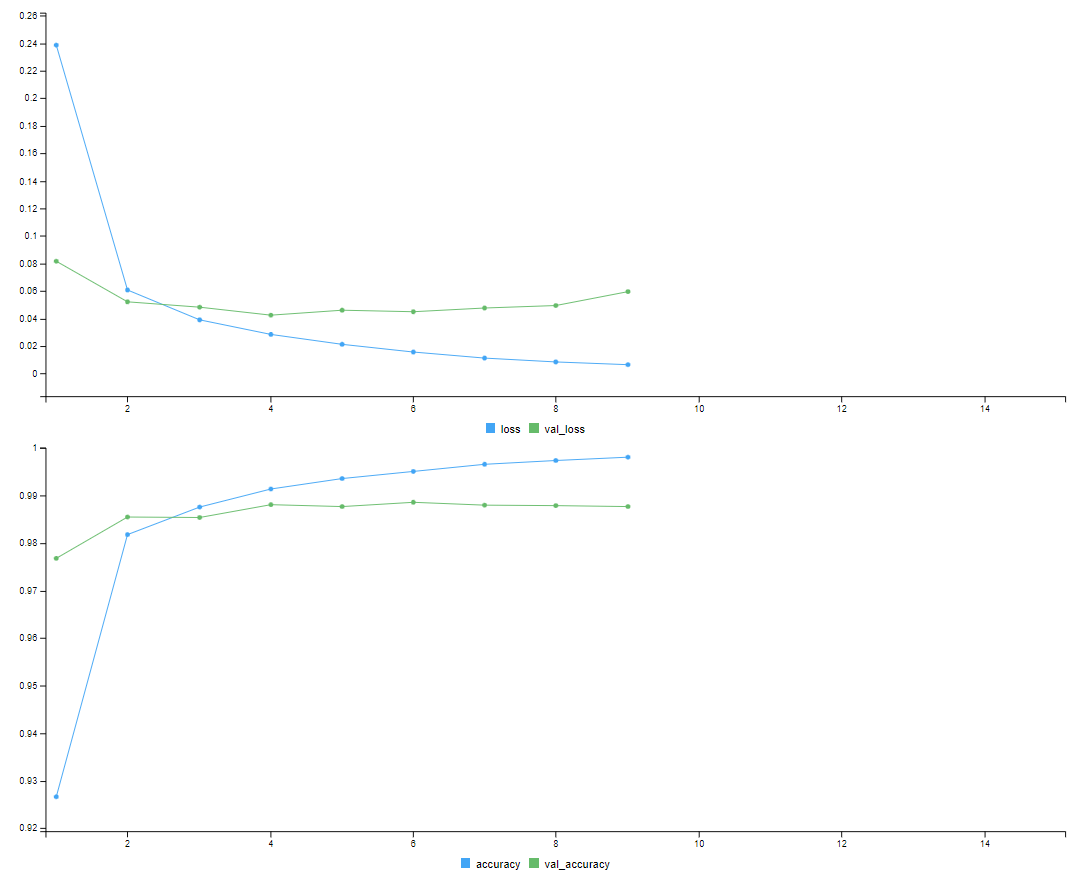
\includegraphics[width=\maxwidth]{model1} 
\end{knitrout}
\subsection{1.5}
Now we test different hyper parameter values. The three hyper parameter I have chosen are the kernel size for the convolutional layers, the learning rate for the optimizer,  and the Weight decay coefficient for the $L_2$ regularizer. The following code is structured such that using the function \texttt{build\_model()} together with \texttt{call\_existing\_model()} samples new values for the hyper parameters and compiles a model, which is later fitted in the main \texttt{randomSearch()} function. The rest of the code is mostly to print the output and get the model attributes for each iteration.

\begin{knitrout}
\definecolor{shadecolor}{rgb}{0.969, 0.969, 0.969}\color{fgcolor}\begin{kframe}
\begin{alltt}
  \hlcom{# function to return a compiled model given hyper parameters}
\hlstd{call_existing_model} \hlkwb{<-}  \hlkwa{function}\hlstd{(}\hlkwc{kernel_size}\hlstd{,} \hlkwc{weight_decay}\hlstd{,} \hlkwc{lr}\hlstd{) \{}
\hlstd{model} \hlkwb{<-} \hlkwd{keras_model_sequential}\hlstd{()} \hlopt
  \hlkwd{layer_conv_2d}\hlstd{(}\hlkwc{filters} \hlstd{=} \hlnum{32}\hlstd{,} \hlkwc{kernel_size} \hlstd{= kernel_size,} \hlkwc{activation} \hlstd{=} \hlstr{'relu'}\hlstd{,}
                \hlkwc{kernel_regularizer} \hlstd{=} \hlkwd{regularizer_l2}\hlstd{(weight_decay),}
                \hlkwc{input_shape} \hlstd{=} \hlkwd{c}\hlstd{(}\hlnum{28}\hlstd{,} \hlnum{28}\hlstd{,} \hlnum{1}\hlstd{))} \hlopt
  \hlkwd{layer_max_pooling_2d}\hlstd{(}\hlkwc{pool_size} \hlstd{=} \hlkwd{c}\hlstd{(}\hlnum{2}\hlstd{,} \hlnum{2}\hlstd{))} \hlopt
  \hlkwd{layer_conv_2d}\hlstd{(}\hlkwc{filters} \hlstd{=} \hlnum{32}\hlstd{,} \hlkwc{kernel_size} \hlstd{= kernel_size,} \hlkwc{activation} \hlstd{=} \hlstr{'relu'}\hlstd{,}
                \hlkwc{kernel_regularizer} \hlstd{=} \hlkwd{regularizer_l2}\hlstd{(weight_decay))} \hlopt
  \hlkwd{layer_flatten}\hlstd{()} \hlopt
  \hlkwd{layer_dense}\hlstd{(}\hlkwc{units} \hlstd{=} \hlnum{32}\hlstd{,} \hlkwc{activation} \hlstd{=} \hlstr{'relu'}\hlstd{,}
              \hlkwc{kernel_regularizer} \hlstd{=} \hlkwd{regularizer_l2}\hlstd{(weight_decay))} \hlopt
  \hlkwd{layer_dense}\hlstd{(}\hlkwc{units} \hlstd{=} \hlnum{10}\hlstd{,} \hlkwc{activation} \hlstd{=} \hlstr{'softmax'}\hlstd{)}

\hlstd{model} \hlopt
 \hlkwd{compile}\hlstd{(}
  \hlkwc{optimizer} \hlstd{=} \hlkwd{optimizer_rmsprop}\hlstd{(}\hlkwc{learning_rate}\hlstd{=lr),}
  \hlkwc{loss} \hlstd{=} \hlstr{'categorical_crossentropy'}\hlstd{,}
  \hlkwc{metrics} \hlstd{=} \hlkwd{c}\hlstd{(}\hlstr{'accuracy'}\hlstd{)}
\hlstd{)}
\hlkwd{return}\hlstd{(model)}
\hlstd{\}}

\hlcom{#Function to sample hyperparameters and then build model}
\hlstd{build_model} \hlkwb{<-} \hlkwa{function}\hlstd{()\{}
  \hlstd{kernel_int} \hlkwb{<-} \hlkwd{sample}\hlstd{(}\hlnum{2}\hlopt{:}\hlnum{10}\hlstd{,} \hlkwc{size}\hlstd{=}\hlnum{1}\hlstd{)} \hlcom{#sampling random integers 2-10}
  \hlstd{kernel_size} \hlkwb{<-} \hlkwd{c}\hlstd{(kernel_int, kernel_int)}

  \hlstd{weight_decay} \hlkwb{<-} \hlkwd{runif}\hlstd{(}\hlkwc{n}\hlstd{=}\hlnum{1}\hlstd{,} \hlkwc{min}\hlstd{=}\hlnum{0.0001}\hlstd{,} \hlkwc{max}\hlstd{=} \hlnum{0.1}\hlstd{)}
    \hlstd{lr} \hlkwb{<-} \hlkwd{runif}\hlstd{(}\hlkwc{n}\hlstd{=}\hlnum{1}\hlstd{,} \hlkwc{min}\hlstd{=} \hlnum{0.0001}\hlstd{,} \hlkwc{max}\hlstd{=}\hlnum{0.01}\hlstd{)}

  \hlstd{model} \hlkwb{<-} \hlkwd{call_existing_model}\hlstd{(}\hlkwc{kernel_size} \hlstd{= kernel_size,}
                               \hlkwc{weight_decay}\hlstd{=weight_decay,}
                               \hlkwc{lr}\hlstd{=lr)}
  \hlkwd{return}\hlstd{(model)}
\hlstd{\}}


\hlcom{#function to obtain the values of the hyperparameters}
\hlcom{#this assumes that the hyper parameters are the same for the different layers}
\hlcom{#and thus just indexing the first layer}
 \hlstd{hyperparameters_summary} \hlkwb{<-} \hlkwa{function}\hlstd{(}\hlkwc{model}\hlstd{)\{}
   \hlstd{layers_configs} \hlkwb{<-} \hlkwd{lapply}\hlstd{(model}\hlopt{$}\hlstd{layers,} \hlkwa{function}\hlstd{(}\hlkwc{layer}\hlstd{)\{}
     \hlstd{layer}\hlopt{$}\hlkwd{get_config}\hlstd{()}
   \hlstd{\})}
   \hlstd{parameter_vals} \hlkwb{<-} \hlkwd{list}\hlstd{()}
   \hlstd{kernel_int} \hlkwb{<-} \hlstd{layers_configs[[}\hlnum{1}\hlstd{]]}\hlopt{$}\hlstd{kernel_size[[}\hlnum{1}\hlstd{]]}
   \hlstd{kernel_size} \hlkwb{<-} \hlkwd{c}\hlstd{(kernel_int, kernel_int)}
   \hlstd{weight_decay} \hlkwb{<-} \hlstd{layers_configs[[}\hlnum{1}\hlstd{]]}\hlopt{$}\hlstd{kernel_regularizer}\hlopt{$}\hlstd{config}\hlopt{$}\hlstd{l2}

   \hlstd{learning_rate} \hlkwb{<-} \hlstd{model}\hlopt{$}\hlstd{optimizer}\hlopt{$}\hlkwd{get_config}\hlstd{()}\hlopt{$}\hlstd{learning_rate}

  \hlstd{parameter_vals} \hlkwb{<-} \hlkwd{list}\hlstd{(}\hlstr{"kernel_size"} \hlstd{= kernel_size,}
                         \hlstr{"weight_decay"} \hlstd{= weight_decay,}
                         \hlstr{"learning_rate"} \hlstd{= learning_rate )}
   \hlkwd{return}\hlstd{(parameter_vals)}
 \hlstd{\}}

 \hlcom{#just  a wrapper to fit a model}
 \hlstd{fit_model} \hlkwb{<-} \hlkwa{function}\hlstd{(}\hlkwc{model}\hlstd{,} \hlkwc{x_train}\hlstd{,} \hlkwc{y_train}\hlstd{,} \hlkwc{epochs}\hlstd{,} \hlkwc{batch_size}\hlstd{,}
                       \hlkwc{validation_split}\hlstd{,}\hlkwc{...}\hlstd{)\{}
   \hlstd{model} \hlopt
   \hlkwd{fit}\hlstd{(x_train, y_train,}
       \hlkwc{epochs}\hlstd{=epochs,}
       \hlkwc{batch_size}\hlstd{=batch_size,}
       \hlkwc{validation_split}\hlstd{=validation_split,}
       \hlstd{...)}
 \hlstd{\}}

 \hlcom{#the print functions are only used withing the  RandomSearch function}
 \hlstd{print_summary} \hlkwb{<-} \hlkwa{function}\hlstd{(}\hlkwc{hyperparameters_summary}\hlstd{)\{}
   \hlkwd{cat}\hlstd{(}\hlstr{"Current Kernel size is "}\hlstd{, hyperparameters_summary}\hlopt{$}\hlstd{kernel_size,} \hlstr{"\textbackslash{}n"}\hlstd{)}
   \hlkwd{cat}\hlstd{(}\hlstr{"Current weight decay is:"}\hlstd{, hyperparameters_summary}\hlopt{$}\hlstd{weight_decay,} \hlstr{"\textbackslash{}n"}\hlstd{)}
   \hlkwd{cat}\hlstd{(}\hlstr{"Current learning rate is"}\hlstd{, hyperparameters_summary}\hlopt{$}\hlstd{learning_rate,} \hlstr{"\textbackslash{}n"}\hlstd{)}
 \hlstd{\}}

 \hlcom{#function to return the model_history results }
 \hlcom{#for simplicity sake this does not consider early stopping and just returns}
 \hlcom{# the last epoch results}
 \hlstd{get_model_results} \hlkwb{<-} \hlkwa{function}\hlstd{(}\hlkwc{model_history}\hlstd{)\{}
   \hlstd{n_epochs} \hlkwb{<-} \hlstd{model_history}\hlopt{$}\hlstd{params}\hlopt{$}\hlstd{epochs}
   \hlstd{loss} \hlkwb{<-} \hlstd{model_history}\hlopt{$}\hlstd{metrics}\hlopt{$}\hlstd{loss[n_epochs]}
   \hlstd{accuracy} \hlkwb{<-} \hlstd{model_history}\hlopt{$}\hlstd{metrics}\hlopt{$}\hlstd{accuracy[n_epochs]}
   \hlstd{val_loss} \hlkwb{<-} \hlstd{model_history}\hlopt{$}\hlstd{metrics}\hlopt{$}\hlstd{val_loss[n_epochs]}
   \hlstd{val_accuracy} \hlkwb{<-} \hlstd{model_history}\hlopt{$}\hlstd{metrics}\hlopt{$}\hlstd{val_accuracy[n_epochs]}
   \hlstd{results} \hlkwb{<-} \hlkwd{list}\hlstd{(}\hlstr{"loss"}\hlstd{= loss,} \hlstr{"accuracy"} \hlstd{= accuracy,}
                   \hlstr{"val_loss"} \hlstd{= val_loss,} \hlstr{"val_accuracy"} \hlstd{= val_accuracy)}
   \hlkwd{return}\hlstd{(results)}
 \hlstd{\}}


\hlstd{print_current_best} \hlkwb{<-} \hlkwa{function}\hlstd{(}\hlkwc{current_best_list}\hlstd{)\{}
  \hlkwd{cat}\hlstd{(}\hlstr{"Current best model is model no."}\hlstd{, current_best_list}\hlopt{$}\hlstd{index,}
      \hlstr{" with the following hyperparameters: \textbackslash{}n"}\hlstd{)}
  \hlkwd{cat}\hlstd{(}\hlstr{"Hyperparameters:  \textbackslash{}n"}\hlstd{,} \hlstr{"Kernel_size : "}\hlstd{,}
      \hlstd{current_best_list}\hlopt{$}\hlstd{model_summary}\hlopt{$}\hlstd{kernel_size,} \hlstr{"\textbackslash{}n"} \hlstd{)}
  \hlkwd{cat}\hlstd{(}\hlstr{"weight decay: "}\hlstd{, current_best_list}\hlopt{$}\hlstd{model_summary}\hlopt{$}\hlstd{weight_decay,} \hlstr{"\textbackslash{}n"} \hlstd{)}
  \hlkwd{cat}\hlstd{(}\hlstr{"learning rate:"}\hlstd{, current_best_list}\hlopt{$}\hlstd{model_summary}\hlopt{$}\hlstd{learning_rate,} \hlstr{"\textbackslash{}n"}\hlstd{)}
  \hlkwd{cat}\hlstd{(}\hlstr{"Validation accuracy:"}\hlstd{, current_best_list}\hlopt{$}\hlstd{model_results}\hlopt{$}\hlstd{val_accuracy,} \hlstr{"\textbackslash{}n"}\hlstd{)}
\hlstd{\}}

\hlstd{print_new_iter} \hlkwb{<-} \hlkwa{function}\hlstd{(}\hlkwc{iter}\hlstd{)\{}
  \hlstd{line_breaks} \hlkwb{<-} \hlkwd{strrep}\hlstd{(}\hlstr{"*"}\hlstd{,} \hlnum{25}\hlstd{)}
  \hlkwd{cat}\hlstd{(line_breaks,} \hlstr{"\textbackslash{}n"}\hlstd{,} \hlstr{"New Model! \textbackslash{}n"}\hlstd{, line_breaks,} \hlstr{"\textbackslash{}n"} \hlstd{)}
  \hlkwd{cat}\hlstd{(}\hlstr{"Current model number is:"}\hlstd{, iter,} \hlstr{"\textbackslash{}n"}\hlstd{)}
\hlstd{\}}

\hlcom{#main function to implement the RandomSearch method}
\hlstd{RandomSearch} \hlkwb{<-} \hlkwa{function}\hlstd{(}\hlkwc{iterations}\hlstd{,} \hlkwc{x_train}\hlstd{,} \hlkwc{y_train}\hlstd{,} \hlkwc{epochs}\hlstd{,}
                         \hlkwc{batch_size}\hlstd{,} \hlkwc{validation_split}\hlstd{,} \hlkwc{...}\hlstd{)\{}
  \hlstd{all_models} \hlkwb{<-} \hlkwd{list}\hlstd{()}
  \hlstd{current_best} \hlkwb{<-} \hlkwd{list}\hlstd{()}
  \hlstd{index} \hlkwb{<-} \hlnum{0}
  \hlkwa{for} \hlstd{(i} \hlkwa{in} \hlnum{1}\hlopt{:}\hlstd{iterations)\{}
    \hlstd{index} \hlkwb{<-} \hlstd{index} \hlopt{+} \hlnum{1}
    \hlstd{model} \hlkwb{<-} \hlkwd{build_model}\hlstd{()}
    \hlcom{#print model summary}
    \hlstd{hyper_summary} \hlkwb{<-} \hlkwd{hyperparameters_summary}\hlstd{(model)}
    \hlkwd{print_new_iter}\hlstd{(}\hlkwc{iter}\hlstd{=index)}
    \hlkwd{print_summary}\hlstd{(hyper_summary)}


    \hlstd{model_history} \hlkwb{<-} \hlkwd{fit_model}\hlstd{(model,  x_train, y_train,} \hlkwc{epochs}\hlstd{=epochs,}
                         \hlkwc{batch_size}\hlstd{=batch_size,}
                         \hlkwc{validation_split}\hlstd{=validation_split)}

    \hlstd{model_results} \hlkwb{<-} \hlkwd{get_model_results}\hlstd{(model_history)}

    \hlstd{iteration_results} \hlkwb{<-} \hlkwd{list}\hlstd{(}\hlstr{"model"} \hlstd{= model,}
                              \hlstr{"model_summary"} \hlstd{= hyper_summary,}
                              \hlstr{"model_history"} \hlstd{= model_history,}
                              \hlstr{"model_results"} \hlstd{= model_results,}
                              \hlstr{"index"} \hlstd{= index)}
    \hlstd{all_models[[i]]} \hlkwb{<-} \hlstd{iteration_results}

    \hlkwa{if}\hlstd{(index}\hlopt{==}\hlnum{1}\hlstd{) \{}
      \hlstd{current_best} \hlkwb{<-} \hlstd{iteration_results\}} \hlkwa{else}\hlstd{\{}
        \hlstd{cur_best_acc} \hlkwb{<-} \hlstd{current_best}\hlopt{$}\hlstd{model_results}\hlopt{$}\hlstd{val_accuracy}
        \hlstd{iteration_accuracy} \hlkwb{<-} \hlstd{model_results}\hlopt{$}\hlstd{val_accuracy}
        \hlkwa{if}\hlstd{(iteration_accuracy} \hlopt{>} \hlstd{cur_best_acc)\{}
          \hlstd{current_best} \hlkwb{<-} \hlstd{iteration_results}
        \hlstd{\}}
      \hlstd{\}}
    \hlkwd{print_current_best}\hlstd{(current_best)}

  \hlstd{\}}
 \hlstd{all_results} \hlkwb{<-} \hlkwd{list}\hlstd{(}
    \hlstr{"all_models"} \hlstd{= all_models,}
    \hlstr{"best_model"} \hlstd{= current_best}
  \hlstd{)}
   \hlkwd{plot}\hlstd{(all_results}\hlopt{$}\hlstd{best_model}\hlopt{$}\hlstd{model_history)}
  \hlkwd{return}\hlstd{(all_results)}
\hlstd{\}}
\end{alltt}
\end{kframe}
\end{knitrout}


\begin{knitrout}
\definecolor{shadecolor}{rgb}{0.969, 0.969, 0.969}\color{fgcolor}\begin{kframe}
\begin{alltt}
\hlstd{RS_results} \hlkwb{<-} \hlkwd{RandomSearch}\hlstd{(}\hlkwc{iterations}\hlstd{=}\hlnum{10}\hlstd{,}
             \hlkwc{x_train}\hlstd{=x_train,} \hlkwc{y_train}\hlstd{=y_train,}
             \hlkwc{epochs}\hlstd{=}\hlnum{10}\hlstd{,} \hlkwc{batch_size}\hlstd{=}\hlnum{256}\hlstd{,}
             \hlkwc{validation_split}\hlstd{=}\hlnum{0.2}\hlstd{)}

\hlkwd{plot}\hlstd{(RS_results}\hlopt{$}\hlstd{best_model}\hlopt{$}\hlstd{model_history)}
\end{alltt}
\end{kframe}
\end{knitrout}

Based on the results, the best model was the following: 
\begin{knitrout}
\definecolor{shadecolor}{rgb}{0.969, 0.969, 0.969}\color{fgcolor}\begin{kframe}
\begin{alltt}
RS_results$best_model$model_summary

$kernel_size
[1] 7 7

$weight_decay
[1] 0.009164357

$learning_rate
[1] 0.005879265
\end{alltt}
\end{kframe}
\end{knitrout}

\begin{knitrout}
\definecolor{shadecolor}{rgb}{0.969, 0.969, 0.969}\color{fgcolor}\begin{kframe}
\begin{alltt}
RS_results$best_model$model_results

$loss
[1] 0.2912685

$accuracy
[1] 0.9540833

$val_loss
[1] 0.2386363

$val_accuracy
[1] 0.9706666
\end{alltt}
\end{kframe}
\end{knitrout}

Hence, kernel\_size = (7,7), weight decay = 0.009 and learning rate =0.00059. The validation accuracy was 0.97. 
This validation accuracy was lower than the one obtained in the previous task. However, a pattern was that the accuracy was generally increasing on average after each epoch. Hence, ideally it would have been better to run more epochs, but that would also not be as computationally efficient, which is why it was limited to 10 epochs in this case. 

The full model summary and the results per epoch figure are:

\begin{knitrout}
\definecolor{shadecolor}{rgb}{0.969, 0.969, 0.969}\color{fgcolor}\begin{kframe}
\begin{alltt}
RS_results$best_mode$model

 \hlkwd{Layer} (type)                      Output Shape                Param \hlcom{#   }
================================================================================
 \hlkwd{conv2d_11} (Conv2D)                (None, 22, 22, 32)         1600            
 \hlkwd{max_pooling2d_5} (MaxPooling2D)    (None, 11, 11, 32)         0                 
 \hlkwd{conv2d_10} (Conv2D)                (None, 5, 5, 32)           50208             
 \hlkwd{flatten_5} (Flatten)               (None, 800)                0                 
 \hlkwd{dense_11} (Dense)                  (None, 32)                 25632             
 \hlkwd{dense_10} (Dense)                  (None, 10)                 330               
================================================================================
Total params: \hlkwd{77770} (303.79 KB)
Trainable params: \hlkwd{77770} (303.79 KB)
Non-trainable params: \hlkwd{0} (0.00 Byte)
_____________________________________
\end{alltt}
\end{kframe}
\end{knitrout}


\begin{knitrout}
\definecolor{shadecolor}{rgb}{0.969, 0.969, 0.969}\color{fgcolor}\begin{kframe}
\begin{alltt}
\hlkwd{plot}\hlstd{(RS_results}\hlopt{$}\hlstd{best_model}\hlopt{$}\hlstd{model_history)}
\end{alltt}
\end{kframe}
\end{knitrout}

\begin{knitrout}
\definecolor{shadecolor}{rgb}{0.969, 0.969, 0.969}\color{fgcolor}\begin{kframe}
\begin{alltt}
\hlstd{knitr}\hlopt{::}\hlkwd{include_graphics}\hlstd{(}\hlstr{"best_model.png"}\hlstd{)}
\end{alltt}
\end{kframe}\begin{figure}
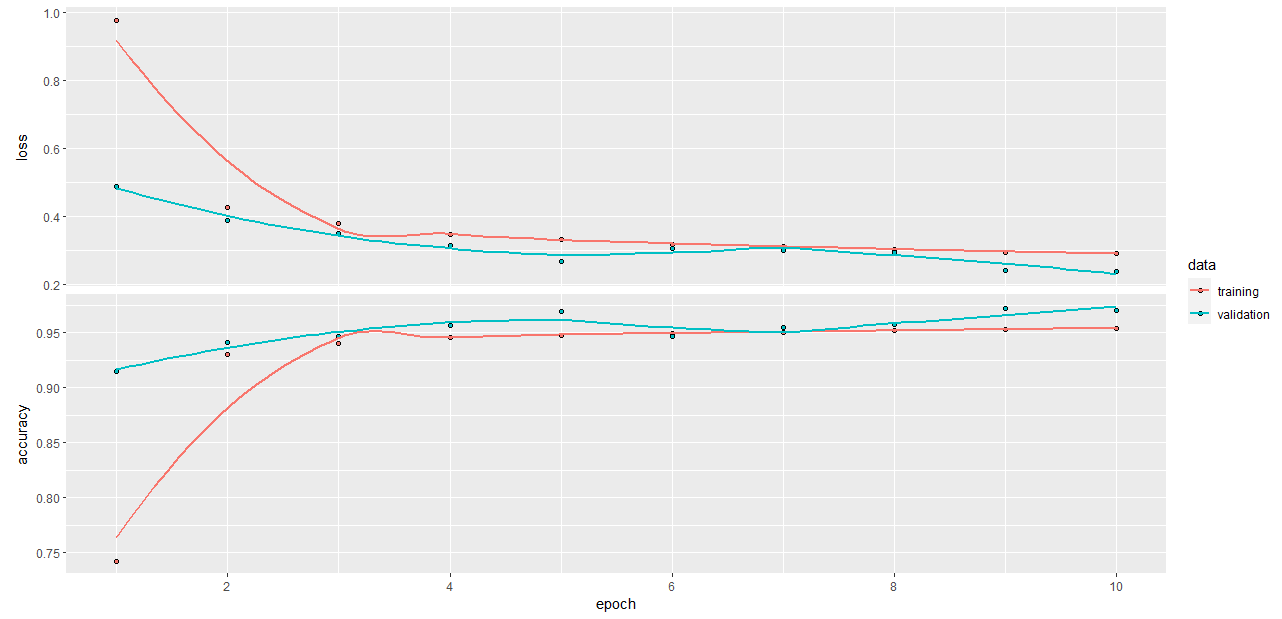
\includegraphics[width=\maxwidth]{best_model} \caption[best model results]{best model results}\label{fig:unnamed-chunk-14}
\end{figure}

\end{knitrout}


\subsection{1.6}
Now we use the cifar data set
\begin{knitrout}
\definecolor{shadecolor}{rgb}{0.969, 0.969, 0.969}\color{fgcolor}\begin{kframe}
\begin{alltt}
\hlstd{cifar10} \hlkwb{<-} \hlkwd{dataset_cifar10}\hlstd{()}

\hlstd{x_train} \hlkwb{<-} \hlstd{cifar10}\hlopt{$}\hlstd{train}\hlopt{$}\hlstd{x}\hlopt{/}\hlnum{255}
\hlstd{x_test} \hlkwb{<-} \hlstd{cifar10}\hlopt{$}\hlstd{test}\hlopt{$}\hlstd{x}\hlopt{/}\hlnum{255}
\hlstd{y_train} \hlkwb{<-} \hlstd{cifar10}\hlopt{$}\hlstd{train}\hlopt{$}\hlstd{y}
\hlstd{y_test} \hlkwb{<-} \hlstd{cifar10}\hlopt{$}\hlstd{test}\hlopt{$}\hlstd{y}
\end{alltt}
\end{kframe}
\end{knitrout}

\begin{knitrout}
\definecolor{shadecolor}{rgb}{0.969, 0.969, 0.969}\color{fgcolor}\begin{kframe}
\begin{alltt}
\hlstd{model_cifar} \hlkwb{<-} \hlkwd{keras_model_sequential}\hlstd{()} \hlopt
  \hlcom{# First hidden 2D convolutional layer}
  \hlkwd{layer_conv_2d}\hlstd{(}
    \hlkwc{filters} \hlstd{=} \hlnum{32}\hlstd{,}
    \hlkwc{kernel_size} \hlstd{=} \hlkwd{c}\hlstd{(}\hlnum{3}\hlstd{,} \hlnum{3}\hlstd{),}
    \hlkwc{padding} \hlstd{=} \hlstr{"valid"}\hlstd{,}
    \hlkwc{input_shape} \hlstd{=} \hlkwd{c}\hlstd{(}\hlnum{32}\hlstd{,} \hlnum{32}\hlstd{,} \hlnum{3}\hlstd{)}
  \hlstd{)} \hlopt

  \hlcom{# Use max pooling}
  \hlkwd{layer_max_pooling_2d}\hlstd{(}\hlkwc{pool_size} \hlstd{=} \hlkwd{c}\hlstd{(}\hlnum{2}\hlstd{,} \hlnum{2}\hlstd{))} \hlopt
  \hlcom{# Second hidden layer}
  \hlkwd{layer_conv_2d}\hlstd{(}\hlkwc{filters} \hlstd{=} \hlnum{64}\hlstd{,} \hlkwc{kernel_size} \hlstd{=} \hlkwd{c}\hlstd{(}\hlnum{3}\hlstd{,} \hlnum{3}\hlstd{),} \hlkwc{padding} \hlstd{=} \hlstr{"valid"}\hlstd{)} \hlopt


  \hlcom{# Use max pooling once more}
  \hlkwd{layer_max_pooling_2d}\hlstd{(}\hlkwc{pool_size} \hlstd{=} \hlkwd{c}\hlstd{(}\hlnum{2}\hlstd{,} \hlnum{2}\hlstd{))} \hlopt

  \hlcom{# Third hidden layer}
  \hlkwd{layer_conv_2d}\hlstd{(}\hlkwc{filters} \hlstd{=} \hlnum{64}\hlstd{,} \hlkwc{kernel_size} \hlstd{=} \hlkwd{c}\hlstd{(}\hlnum{3}\hlstd{,} \hlnum{3}\hlstd{))} \hlopt


  \hlcom{# Flatten max filtered output into feature vector }
  \hlcom{# and feed into dense layer}
  \hlkwd{layer_flatten}\hlstd{()} \hlopt

  \hlcom{# Fourth hidden layer}
  \hlkwd{layer_dense}\hlstd{(}\hlkwc{units} \hlstd{=} \hlnum{64}\hlstd{)} \hlopt


  \hlcom{# Outputs from dense layer are projected onto 10 unit output layer}
  \hlkwd{layer_dense}\hlstd{(}\hlkwc{units} \hlstd{=} \hlnum{10}\hlstd{)}

\hlkwd{summary}\hlstd{(model_cifar)}
\end{alltt}
\begin{verbatim}
Model: "sequential_1"
________________________________________________________________________________
 Layer (type)                       Output Shape                    Param #     
================================================================================
 conv2d_4 (Conv2D)                  (None, 30, 30, 32)              896         
 max_pooling2d_2 (MaxPooling2D)     (None, 15, 15, 32)              0           
 conv2d_3 (Conv2D)                  (None, 13, 13, 64)              18496       
 max_pooling2d_1 (MaxPooling2D)     (None, 6, 6, 64)                0           
 conv2d_2 (Conv2D)                  (None, 4, 4, 64)                36928       
 flatten_1 (Flatten)                (None, 1024)                    0           
 dense_3 (Dense)                    (None, 64)                      65600       
 dense_2 (Dense)                    (None, 10)                      650         
================================================================================
Total params: 122570 (478.79 KB)
Trainable params: 122570 (478.79 KB)
Non-trainable params: 0 (0.00 Byte)
________________________________________________________________________________
\end{verbatim}
\end{kframe}
\end{knitrout}

running it yields:
\begin{knitrout}
\definecolor{shadecolor}{rgb}{0.969, 0.969, 0.969}\color{fgcolor}\begin{kframe}
\begin{alltt}
\hlstd{opt} \hlkwb{<-} \hlkwd{optimizer_adamax}\hlstd{(}\hlkwc{learning_rate} \hlstd{=} \hlkwd{learning_rate_schedule_exponential_decay}\hlstd{(}
  \hlkwc{initial_learning_rate} \hlstd{=} \hlnum{5e-3}\hlstd{,}
  \hlkwc{decay_rate} \hlstd{=} \hlnum{0.96}\hlstd{,}
  \hlkwc{decay_steps} \hlstd{=} \hlnum{1500}\hlstd{,}
  \hlkwc{staircase} \hlstd{=} \hlnum{TRUE}
\hlstd{))}

\hlstd{model_cifar} \hlopt \hlkwd{compile}\hlstd{(}
  \hlkwc{loss} \hlstd{=} \hlkwd{loss_sparse_categorical_crossentropy}\hlstd{(}\hlkwc{from_logits} \hlstd{=} \hlnum{TRUE}\hlstd{),}
  \hlkwc{optimizer} \hlstd{= opt,}
  \hlkwc{metrics} \hlstd{=} \hlstr{"accuracy"}
\hlstd{)}


\hlcom{# Training ----------------------------------------------------------------}
\hlstd{model_cifar} \hlopt \hlkwd{fit}\hlstd{(}
  \hlstd{x_train, y_train,}
  \hlkwc{batch_size} \hlstd{=} \hlnum{128}\hlstd{,}
  \hlkwc{epochs} \hlstd{=} \hlnum{10}\hlstd{,}
  \hlkwc{validation_data} \hlstd{=} \hlkwd{list}\hlstd{(x_test, y_test),}
  \hlkwc{shuffle} \hlstd{=} \hlnum{TRUE}
\hlstd{)}
\end{alltt}
\end{kframe}
\end{knitrout}

\begin{knitrout}
\definecolor{shadecolor}{rgb}{0.969, 0.969, 0.969}\color{fgcolor}\begin{kframe}
\begin{alltt}
Epoch 10/10
391/391 [==============================] - 23s 60ms/step 
- loss: 0.9227 - accuracy: 0.6837 - val_loss: 1.0588 - val_accuracy: 0.6481
\end{alltt}
\end{kframe}
\end{knitrout}

\begin{knitrout}
\definecolor{shadecolor}{rgb}{0.969, 0.969, 0.969}\color{fgcolor}\begin{kframe}
\begin{alltt}
\hlstd{knitr}\hlopt{::}\hlkwd{include_graphics}\hlstd{(}\hlstr{"cifar_model.png"}\hlstd{)}
\end{alltt}
\end{kframe}\begin{figure}
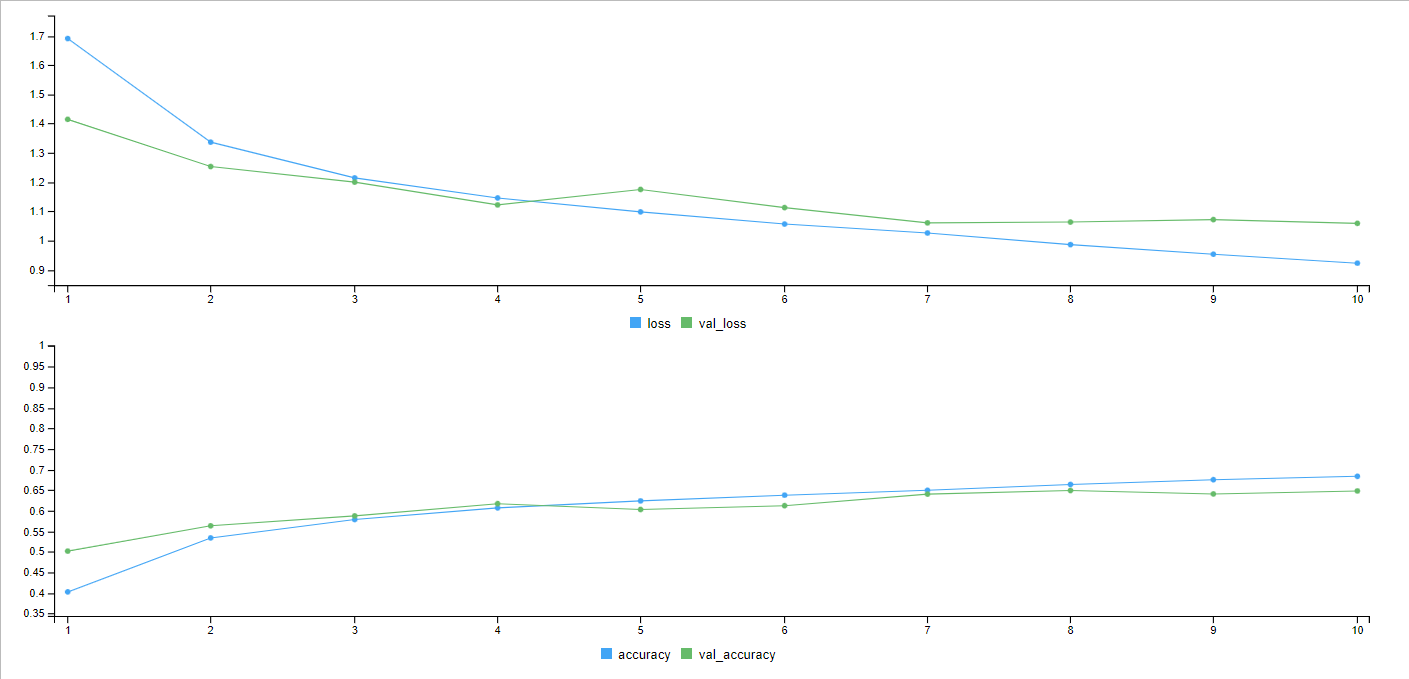
\includegraphics[width=\maxwidth]{cifar_model} \caption[cifar model results]{cifar model results}\label{fig:unnamed-chunk-19}
\end{figure}

\end{knitrout}
Looking at the results, we see that the validation accuracy is rather low compared to before with the mnist data since the accuracy is around 0.65. However, The accuracy was increasing for each epoch and we could probably have gotten it higher if we just ran it for more epochs. 

\subsection{1.7}
Now we visualize one image


\begin{knitrout}
\definecolor{shadecolor}{rgb}{0.969, 0.969, 0.969}\color{fgcolor}\begin{kframe}
\begin{alltt}
\hlkwd{library}\hlstd{(EBImage)}
\hlstd{class_labels} \hlkwb{<-} \hlkwd{c}\hlstd{(}\hlstr{"Airplane"}\hlstd{,} \hlstr{"Car"}\hlstd{,} \hlstr{"Bird"}\hlstd{,} \hlstr{"Cat"}\hlstd{,} \hlstr{"Deer"}\hlstd{,} \hlstr{"Dog"}\hlstd{,}
                  \hlstr{"Frog"}\hlstd{,} \hlstr{"Horse"}\hlstd{,} \hlstr{"Ship"}\hlstd{,} \hlstr{"Truck"}\hlstd{)}
\hlstd{y_factor} \hlkwb{<-} \hlkwd{factor}\hlstd{(y_train,} \hlkwc{levels} \hlstd{=} \hlnum{0}\hlopt{:}\hlnum{9}\hlstd{,} \hlkwc{labels} \hlstd{= class_labels)}

\hlstd{plot_images_2} \hlkwb{<-} \hlkwa{function}\hlstd{(}\hlkwc{idx}\hlstd{,} \hlkwc{x_train}\hlstd{,} \hlkwc{y_train}\hlstd{)\{}
  \hlkwd{par}\hlstd{(}\hlkwc{mfrow}\hlstd{=}\hlkwd{c}\hlstd{(}\hlnum{1}\hlstd{,}\hlnum{2}\hlstd{),} \hlkwc{mar} \hlstd{=} \hlkwd{c}\hlstd{(}\hlnum{4}\hlstd{,} \hlnum{2}\hlstd{,} \hlnum{2}\hlstd{,} \hlnum{2}\hlstd{))}

  \hlstd{fig_img} \hlkwb{<-} \hlkwd{list}\hlstd{()}
  \hlkwa{for} \hlstd{(i} \hlkwa{in} \hlnum{1}\hlopt{:}\hlkwd{length}\hlstd{(idx))\{}
    \hlstd{fig_mat} \hlkwb{<-} \hlstd{x_train[idx[i],,,]}
    \hlstd{fig_img[[i]]} \hlkwb{<-} \hlkwd{normalize}\hlstd{(}\hlkwd{Image}\hlstd{(}\hlkwd{transpose}\hlstd{(fig_mat),} \hlkwc{dim}\hlstd{=}\hlkwd{c}\hlstd{(}\hlnum{32}\hlstd{,}\hlnum{32}\hlstd{,}\hlnum{3}\hlstd{),} \hlkwc{colormode}\hlstd{=}\hlstr{'Color'}\hlstd{))}
    \hlstd{label} \hlkwb{<-} \hlstd{y_factor[idx[i]]}
    \hlkwd{plot}\hlstd{(fig_img[[i]])}
    \hlkwd{title}\hlstd{(}\hlkwc{main}\hlstd{=label)}
  \hlstd{\}}
  \hlkwd{par}\hlstd{(}\hlkwc{mfrow}\hlstd{=}\hlkwd{c}\hlstd{(}\hlnum{1}\hlstd{,}\hlnum{1}\hlstd{))}
\hlstd{\}}
\end{alltt}
\end{kframe}
\end{knitrout}


\begin{knitrout}
\definecolor{shadecolor}{rgb}{0.969, 0.969, 0.969}\color{fgcolor}\begin{kframe}
\begin{alltt}
\hlkwd{plot_images_2}\hlstd{(}\hlkwc{idx} \hlstd{=} \hlkwd{c}\hlstd{(}\hlnum{13}\hlstd{,} \hlnum{37}\hlstd{), x_train, y_train)}
\end{alltt}
\end{kframe}\begin{figure}
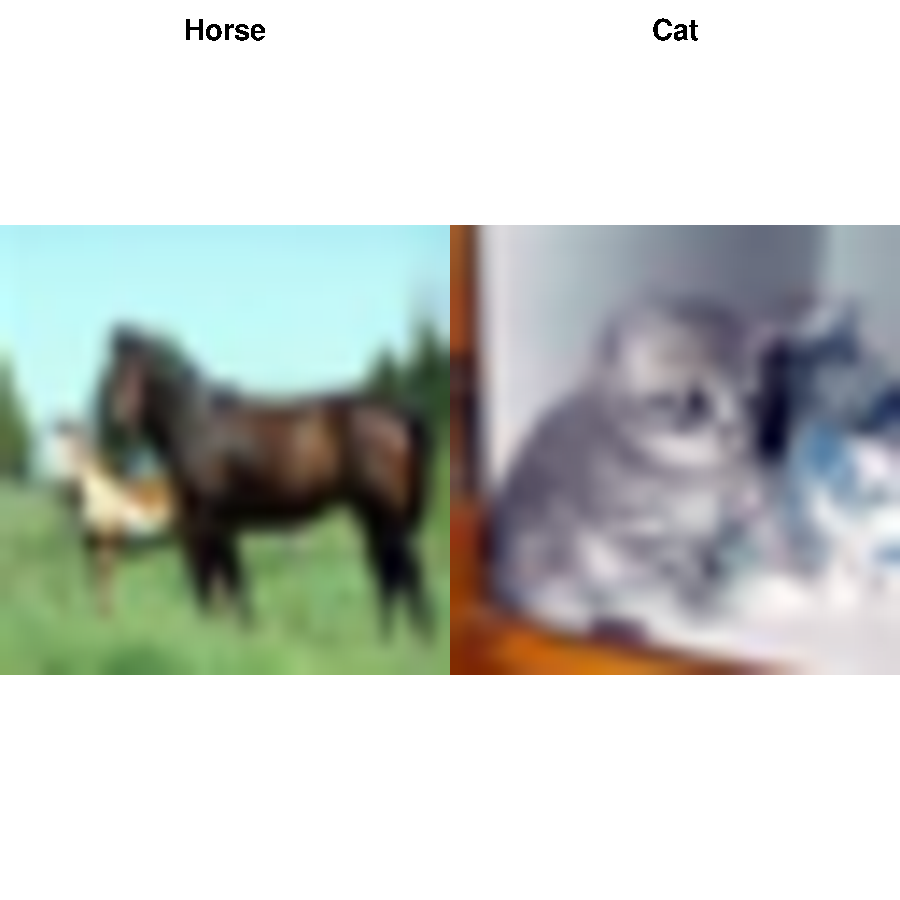
\includegraphics[width=\maxwidth]{figure/unnamed-chunk-21-1} \caption[Images from the cifar data set]{Images from the cifar data set}\label{fig:unnamed-chunk-21}
\end{figure}

\end{knitrout}
\subsection{task 1.8}
The reason we know have 896 parameters is because we know have the input channels the rgb for color, which is equal to 3. Hence, whereas we previously had $(3 \times 3 + 1) \times 32 = 10 \times 320 = 320$  we know have $(3 \times 3 \times 3+ 1) \times 32 = 28 \times 32 = 896$ 

\subsection{task 1.9}
First we start of by adding more hidden layers, both convolutional and dense layers, and increasing the number of hidden unis, which increases the representational capacity of the model. This is so we can potentially overfit. However, due to computational reasons, I will not go all out but simply try adding a relatively small change. We also increase the epochs to 15 to give it more time to converge. 

\begin{knitrout}
\definecolor{shadecolor}{rgb}{0.969, 0.969, 0.969}\color{fgcolor}\begin{kframe}
\begin{alltt}
\hlstd{model_cifar2} \hlkwb{<-} \hlkwd{keras_model_sequential}\hlstd{()} \hlopt
  \hlcom{# First hidden 2D convolutional layer}
  \hlkwd{layer_conv_2d}\hlstd{(}
    \hlkwc{filters} \hlstd{=} \hlnum{32}\hlstd{,}
    \hlkwc{kernel_size} \hlstd{=} \hlkwd{c}\hlstd{(}\hlnum{3}\hlstd{,} \hlnum{3}\hlstd{),}
    \hlkwc{padding} \hlstd{=} \hlstr{"valid"}\hlstd{,}
    \hlkwc{input_shape} \hlstd{=} \hlkwd{c}\hlstd{(}\hlnum{32}\hlstd{,} \hlnum{32}\hlstd{,} \hlnum{3}\hlstd{)}
  \hlstd{)} \hlopt

  \hlcom{# Use max pooling}
  \hlkwd{layer_max_pooling_2d}\hlstd{(}\hlkwc{pool_size} \hlstd{=} \hlkwd{c}\hlstd{(}\hlnum{2}\hlstd{,} \hlnum{2}\hlstd{))} \hlopt
  \hlcom{# Second hidden layer}
  \hlkwd{layer_conv_2d}\hlstd{(}\hlkwc{filters} \hlstd{=} \hlnum{64}\hlstd{,} \hlkwc{kernel_size} \hlstd{=} \hlkwd{c}\hlstd{(}\hlnum{3}\hlstd{,} \hlnum{3}\hlstd{),} \hlkwc{padding} \hlstd{=} \hlstr{"valid"}\hlstd{)} \hlopt

  \hlcom{# Use max pooling once more}
  \hlkwd{layer_max_pooling_2d}\hlstd{(}\hlkwc{pool_size} \hlstd{=} \hlkwd{c}\hlstd{(}\hlnum{2}\hlstd{,} \hlnum{2}\hlstd{))} \hlopt

  \hlcom{# second convulutional hidden layer}
  \hlkwd{layer_conv_2d}\hlstd{(}\hlkwc{filters} \hlstd{=} \hlnum{64}\hlstd{,} \hlkwc{kernel_size} \hlstd{=} \hlkwd{c}\hlstd{(}\hlnum{3}\hlstd{,} \hlnum{3}\hlstd{),} \hlkwc{padding}\hlstd{=}\hlstr{"valid"}\hlstd{)} \hlopt

  \hlcom{#third convulutional hidden layer}
  \hlkwd{layer_conv_2d}\hlstd{(}\hlkwc{filters} \hlstd{=} \hlnum{64}\hlstd{,} \hlkwc{kernel_size} \hlstd{=} \hlkwd{c}\hlstd{(}\hlnum{3}\hlstd{,} \hlnum{3}\hlstd{),} \hlkwc{padding}\hlstd{=}\hlstr{"valid"}\hlstd{)} \hlopt

  \hlcom{# Flatten max filtered output into feature vector }
  \hlcom{# and feed into dense layer}
  \hlkwd{layer_flatten}\hlstd{()} \hlopt

  \hlcom{# Fourth hidden layer}
  \hlkwd{layer_dense}\hlstd{(}\hlkwc{units} \hlstd{=} \hlnum{256}\hlstd{,} \hlkwc{activation} \hlstd{=} \hlstr{"relu"}\hlstd{)} \hlopt

  \hlkwd{layer_dense}\hlstd{(}\hlkwc{units}\hlstd{=}\hlnum{128}\hlstd{,} \hlkwc{activation}\hlstd{=}\hlstr{"relu"}\hlstd{)} \hlopt

  \hlcom{# 10 unit output layer}
  \hlkwd{layer_dense}\hlstd{(}\hlkwc{units} \hlstd{=} \hlnum{10}\hlstd{)}

\hlkwd{summary}\hlstd{(model_cifar2)}
\end{alltt}
\begin{verbatim}
Model: "sequential_2"
________________________________________________________________________________
 Layer (type)                       Output Shape                    Param #     
================================================================================
 conv2d_8 (Conv2D)                  (None, 30, 30, 32)              896         
 max_pooling2d_4 (MaxPooling2D)     (None, 15, 15, 32)              0           
 conv2d_7 (Conv2D)                  (None, 13, 13, 64)              18496       
 max_pooling2d_3 (MaxPooling2D)     (None, 6, 6, 64)                0           
 conv2d_6 (Conv2D)                  (None, 4, 4, 64)                36928       
 conv2d_5 (Conv2D)                  (None, 2, 2, 64)                36928       
 flatten_2 (Flatten)                (None, 256)                     0           
 dense_6 (Dense)                    (None, 256)                     65792       
 dense_5 (Dense)                    (None, 128)                     32896       
 dense_4 (Dense)                    (None, 10)                      1290        
================================================================================
Total params: 193226 (754.79 KB)
Trainable params: 193226 (754.79 KB)
Non-trainable params: 0 (0.00 Byte)
________________________________________________________________________________
\end{verbatim}
\end{kframe}
\end{knitrout}

\begin{knitrout}
\definecolor{shadecolor}{rgb}{0.969, 0.969, 0.969}\color{fgcolor}\begin{kframe}
\begin{alltt}
\hlstd{model_cifar2} \hlopt \hlkwd{compile}\hlstd{(}
  \hlkwc{loss} \hlstd{=} \hlkwd{loss_sparse_categorical_crossentropy}\hlstd{(}\hlkwc{from_logits} \hlstd{=} \hlnum{TRUE}\hlstd{),}
  \hlkwc{optimizer} \hlstd{= opt,}
  \hlkwc{metrics} \hlstd{=} \hlstr{"accuracy"}
\hlstd{)}


\hlcom{# Training ----------------------------------------------------------------}
\hlstd{model_cifar2} \hlopt \hlkwd{fit}\hlstd{(}
  \hlstd{x_train, y_train,}
  \hlkwc{batch_size} \hlstd{=} \hlnum{128}\hlstd{,}
  \hlkwc{epochs} \hlstd{=} \hlnum{15}\hlstd{,}
  \hlkwc{validation_data} \hlstd{=} \hlkwd{list}\hlstd{(x_test, y_test),}
  \hlkwc{shuffle} \hlstd{=} \hlnum{TRUE}\hlstd{,}
  \hlkwc{callbacks} \hlstd{=} \hlkwd{list}\hlstd{(}\hlkwd{callback_early_stopping}\hlstd{(}\hlkwc{patience} \hlstd{=} \hlnum{5}\hlstd{,} \hlkwc{monitor}\hlstd{=}\hlstr{"val_loss"}\hlstd{))}
\hlstd{)}
\end{alltt}
\end{kframe}
\end{knitrout}

The results are:
\begin{knitrout}
\definecolor{shadecolor}{rgb}{0.969, 0.969, 0.969}\color{fgcolor}\begin{kframe}
\begin{alltt}
Epoch 8/15
391/391 [==============================] - 25s 64ms/step
- loss: 0.6989 - accuracy: 0.7521 - val_loss: 0.8948 - val_accuracy: 0.7108
\end{alltt}
\end{kframe}
\end{knitrout}


\begin{knitrout}
\definecolor{shadecolor}{rgb}{0.969, 0.969, 0.969}\color{fgcolor}\begin{kframe}
\begin{alltt}
\hlstd{knitr}\hlopt{::}\hlkwd{include_graphics}\hlstd{(}\hlstr{"cifar_model_2.png"}\hlstd{)}
\end{alltt}
\end{kframe}\begin{figure}
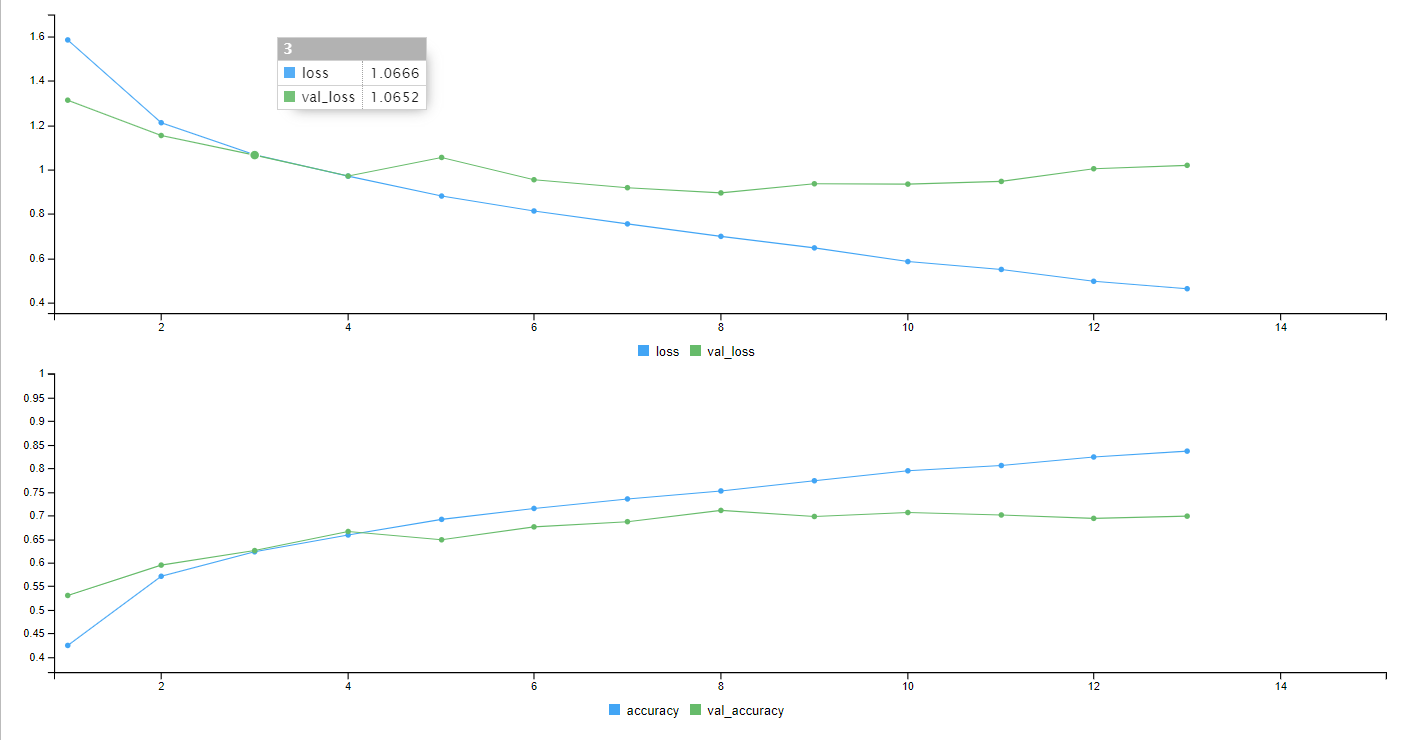
\includegraphics[width=\maxwidth]{cifar_model_2} \caption[Results for second cifar model]{Results for second cifar model}\label{fig:unnamed-chunk-25}
\end{figure}

\end{knitrout}

Looking at the results, it ended at epoch 13 due to the early stopping. The best results were from epoch 8:


The accuracy improved slightly to 0.71

For the next model, we increase the batch size, since a batch with more samples results in more informative gradients with lower variance, while also being more computationally efficient. We also add implicit zero padding to keep the representation size large while also increasing the convolution kernel width to increase the number of parameters in the model . Furthermore, as inspired by the linked guide on the tensorflow webpage for this data set. we can add \texttt{layer\_activation\_leaky\_relu(0.1)} which will allow a small, non-zero gradient when the input is negative and is supposed to helps prevent neurons becoming inactive and stop learning while training. We also increase the number of epochs little bit again and I will tune the learning rate manually as to lower it after 10 epochs, since an improper learning rate will result in a model with low effective capacity.



\begin{knitrout}
\definecolor{shadecolor}{rgb}{0.969, 0.969, 0.969}\color{fgcolor}\begin{kframe}
\begin{alltt}
\hlstd{model_cifar3} \hlkwb{<-} \hlkwd{keras_model_sequential}\hlstd{()} \hlopt
  \hlcom{# First hidden 2D convolutional layer}
  \hlkwd{layer_conv_2d}\hlstd{(}
    \hlkwc{filters} \hlstd{=} \hlnum{32}\hlstd{,}
    \hlkwc{kernel_size} \hlstd{=} \hlkwd{c}\hlstd{(}\hlnum{3}\hlstd{,} \hlnum{3}\hlstd{),}
    \hlkwc{padding} \hlstd{=} \hlstr{"valid"}\hlstd{,}
    \hlkwc{input_shape} \hlstd{=} \hlkwd{c}\hlstd{(}\hlnum{32}\hlstd{,} \hlnum{32}\hlstd{,} \hlnum{3}\hlstd{)}
  \hlstd{)} \hlopt

  \hlcom{# Use max pooling}
  \hlkwd{layer_max_pooling_2d}\hlstd{(}\hlkwc{pool_size} \hlstd{=} \hlkwd{c}\hlstd{(}\hlnum{2}\hlstd{,} \hlnum{2}\hlstd{))} \hlopt
  \hlcom{# Second hidden layer}
  \hlkwd{layer_conv_2d}\hlstd{(}\hlkwc{filters} \hlstd{=} \hlnum{64}\hlstd{,} \hlkwc{kernel_size} \hlstd{=} \hlkwd{c}\hlstd{(}\hlnum{5}\hlstd{,} \hlnum{5}\hlstd{),} \hlkwc{padding} \hlstd{=} \hlstr{"same"}\hlstd{)} \hlopt
  \hlkwd{layer_activation_leaky_relu}\hlstd{(}\hlnum{0.1}\hlstd{)} \hlopt
  \hlcom{# Use max pooling once more}
  \hlkwd{layer_max_pooling_2d}\hlstd{(}\hlkwc{pool_size} \hlstd{=} \hlkwd{c}\hlstd{(}\hlnum{2}\hlstd{,} \hlnum{2}\hlstd{))} \hlopt

  \hlcom{# second convulutional hidden layer}
  \hlkwd{layer_conv_2d}\hlstd{(}\hlkwc{filters} \hlstd{=} \hlnum{64}\hlstd{,} \hlkwc{kernel_size} \hlstd{=} \hlkwd{c}\hlstd{(}\hlnum{5}\hlstd{,} \hlnum{5}\hlstd{),} \hlkwc{padding}\hlstd{=}\hlstr{"same"}\hlstd{)} \hlopt
  \hlkwd{layer_activation_leaky_relu}\hlstd{(}\hlnum{0.1}\hlstd{)} \hlopt

  \hlcom{#third convulutional hidden layer}
  \hlkwd{layer_conv_2d}\hlstd{(}\hlkwc{filters} \hlstd{=} \hlnum{64}\hlstd{,} \hlkwc{kernel_size} \hlstd{=} \hlkwd{c}\hlstd{(}\hlnum{5}\hlstd{,} \hlnum{5}\hlstd{),} \hlkwc{padding}\hlstd{=}\hlstr{"same"}\hlstd{)} \hlopt
  \hlkwd{layer_activation_leaky_relu}\hlstd{(}\hlnum{0.1}\hlstd{)} \hlopt

  \hlcom{# Flatten max filtered output into feature vector }
  \hlcom{# and feed into dense layer}
  \hlkwd{layer_flatten}\hlstd{()} \hlopt

  \hlcom{# Fourth hidden layer}
  \hlkwd{layer_dense}\hlstd{(}\hlkwc{units} \hlstd{=} \hlnum{256}\hlstd{,} \hlkwc{activation} \hlstd{=} \hlstr{"relu"}\hlstd{)} \hlopt

  \hlkwd{layer_dense}\hlstd{(}\hlkwc{units}\hlstd{=}\hlnum{128}\hlstd{,} \hlkwc{activation}\hlstd{=}\hlstr{"relu"}\hlstd{)} \hlopt

  \hlcom{# 10 unit output layer}
  \hlkwd{layer_dense}\hlstd{(}\hlkwc{units} \hlstd{=} \hlnum{10}\hlstd{)}

\hlkwd{print}\hlstd{(model_cifar3)}
\end{alltt}
\begin{verbatim}
Model: "sequential_3"
________________________________________________________________________________
 Layer (type)                       Output Shape                    Param #     
================================================================================
 conv2d_12 (Conv2D)                 (None, 30, 30, 32)              896         
 max_pooling2d_6 (MaxPooling2D)     (None, 15, 15, 32)              0           
 conv2d_11 (Conv2D)                 (None, 15, 15, 64)              51264       
 leaky_re_lu_2 (LeakyReLU)          (None, 15, 15, 64)              0           
 max_pooling2d_5 (MaxPooling2D)     (None, 7, 7, 64)                0           
 conv2d_10 (Conv2D)                 (None, 7, 7, 64)                102464      
 leaky_re_lu_1 (LeakyReLU)          (None, 7, 7, 64)                0           
 conv2d_9 (Conv2D)                  (None, 7, 7, 64)                102464      
 leaky_re_lu (LeakyReLU)            (None, 7, 7, 64)                0           
 flatten_3 (Flatten)                (None, 3136)                    0           
 dense_9 (Dense)                    (None, 256)                     803072      
 dense_8 (Dense)                    (None, 128)                     32896       
 dense_7 (Dense)                    (None, 10)                      1290        
================================================================================
Total params: 1094346 (4.17 MB)
Trainable params: 1094346 (4.17 MB)
Non-trainable params: 0 (0.00 Byte)
________________________________________________________________________________
\end{verbatim}
\end{kframe}
\end{knitrout}


\begin{knitrout}
\definecolor{shadecolor}{rgb}{0.969, 0.969, 0.969}\color{fgcolor}\begin{kframe}
\begin{alltt}
\hlstd{model_cifar3} \hlopt \hlkwd{compile}\hlstd{(}
  \hlkwc{optimizer} \hlstd{=} \hlstr{'RMSprop'}\hlstd{,}
  \hlkwc{loss} \hlstd{=} \hlkwd{loss_sparse_categorical_crossentropy}\hlstd{(}\hlkwc{from_logits} \hlstd{=} \hlnum{TRUE}\hlstd{),}
  \hlkwc{metrics} \hlstd{=} \hlkwd{c}\hlstd{(}\hlstr{'accuracy'}\hlstd{)}
\hlstd{)}


\hlstd{Scheduler} \hlkwb{<-} \hlkwa{function}\hlstd{(}\hlkwc{epoch}\hlstd{,} \hlkwc{lr}\hlstd{) \{}
  \hlkwa{if} \hlstd{(epoch} \hlopt{<} \hlnum{10}\hlstd{) \{}
    \hlkwd{return}\hlstd{(lr)}
  \hlstd{\}} \hlkwa{else} \hlstd{\{}
    \hlkwd{return}\hlstd{(lr} \hlopt{*} \hlkwd{exp}\hlstd{(}\hlopt{-}\hlnum{0.1}\hlstd{))}
  \hlstd{\}}
\hlstd{\}}

\hlstd{callback_list} \hlkwb{=} \hlkwd{list}\hlstd{(}\hlkwd{callback_early_stopping}\hlstd{(}\hlkwc{patience} \hlstd{=} \hlnum{5}\hlstd{),}
                     \hlkwd{callback_learning_rate_scheduler}\hlstd{(Scheduler))}

\hlstd{history_cifar_3} \hlkwb{<-} \hlstd{model_cifar3} \hlopt
  \hlkwd{fit}\hlstd{(}
  \hlstd{x_train, y_train,}
  \hlkwc{epochs} \hlstd{=} \hlnum{20} \hlstd{,}\hlkwc{batch_size} \hlstd{=} \hlnum{512}\hlstd{,}
  \hlkwc{validation_data} \hlstd{=} \hlkwd{list}\hlstd{(x_test, y_test),}
    \hlkwc{shuffle} \hlstd{=} \hlnum{TRUE}\hlstd{,}
  \hlkwc{callbacks} \hlstd{=callback_list)}
\end{alltt}
\end{kframe}
\end{knitrout}

And the results are:

\begin{knitrout}
\definecolor{shadecolor}{rgb}{0.969, 0.969, 0.969}\color{fgcolor}\begin{kframe}
\begin{alltt}
98/98 [==============================] - 61s 620ms/step 
- loss: 0.6635 - accuracy: 0.7688 - val_loss: 0.8182 - val_accuracy: 0.7230 
- lr: 0.0010
\end{alltt}
\end{kframe}
\end{knitrout}

\begin{knitrout}
\definecolor{shadecolor}{rgb}{0.969, 0.969, 0.969}\color{fgcolor}\begin{kframe}
\begin{alltt}
\hlstd{knitr}\hlopt{::}\hlkwd{include_graphics}\hlstd{(}\hlstr{"cifar_model_3.png"}\hlstd{)}
\end{alltt}
\end{kframe}\begin{figure}
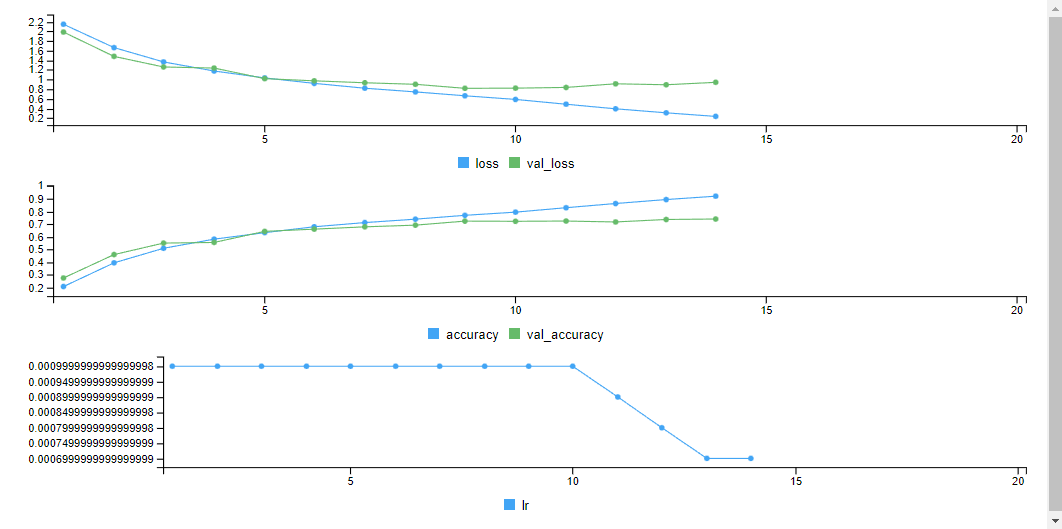
\includegraphics[width=\maxwidth]{cifar_model_3} \caption[Results for the third model]{Results for the third model}\label{fig:unnamed-chunk-29}
\end{figure}

\end{knitrout}
This also stopped early. The validation accuracy was 0.72 and hence a small improvement, although very marginally. 


Next, we can implement some regularization techniques. This will negatively affect the model fit on the training data, but with the aim of making if fit better for validation. More specifically, we will implement the L2 regularization which adds to the a cost to the models loss function of having large weights. Here we simply use the default value of 0.01 since I do not want to test multiple values due to computational reasons.  Furthermore, we will also apply dropout to the layers which works by randomly dropping out a number of the output features of the layers during the training. lastly we can add normalization for the dense layer by normalizing the input of the layer, which can improve the generalization. 

\begin{knitrout}
\definecolor{shadecolor}{rgb}{0.969, 0.969, 0.969}\color{fgcolor}\begin{kframe}
\begin{alltt}
\hlstd{model_cifar4} \hlkwb{<-} \hlkwd{keras_model_sequential}\hlstd{()} \hlopt
  \hlcom{# First hidden 2D convolutional layer}
  \hlkwd{layer_conv_2d}\hlstd{(}
    \hlkwc{filters} \hlstd{=} \hlnum{32}\hlstd{,}
    \hlkwc{kernel_size} \hlstd{=} \hlkwd{c}\hlstd{(}\hlnum{3}\hlstd{,} \hlnum{3}\hlstd{),}
    \hlkwc{padding} \hlstd{=} \hlstr{"valid"}\hlstd{,}
    \hlkwc{input_shape} \hlstd{=} \hlkwd{c}\hlstd{(}\hlnum{32}\hlstd{,} \hlnum{32}\hlstd{,} \hlnum{3}\hlstd{),}
     \hlkwc{kernel_regularizer} \hlstd{=} \hlkwd{regularizer_l2}\hlstd{())} \hlopt

  \hlcom{# Use max pooling}
  \hlkwd{layer_max_pooling_2d}\hlstd{(}\hlkwc{pool_size} \hlstd{=} \hlkwd{c}\hlstd{(}\hlnum{2}\hlstd{,} \hlnum{2}\hlstd{))} \hlopt
   \hlkwd{layer_dropout}\hlstd{(}\hlnum{0.25}\hlstd{)} \hlopt
  \hlcom{# Second hidden layer}
  \hlkwd{layer_conv_2d}\hlstd{(}\hlkwc{filters} \hlstd{=} \hlnum{64}\hlstd{,} \hlkwc{kernel_size} \hlstd{=} \hlkwd{c}\hlstd{(}\hlnum{5}\hlstd{,} \hlnum{5}\hlstd{),} \hlkwc{padding} \hlstd{=} \hlstr{"same"}\hlstd{,}
                \hlkwc{kernel_regularizer} \hlstd{=} \hlkwd{regularizer_l2}\hlstd{())} \hlopt
  \hlkwd{layer_activation_leaky_relu}\hlstd{(}\hlnum{0.1}\hlstd{)} \hlopt
  \hlcom{# Use max pooling once more}
  \hlkwd{layer_max_pooling_2d}\hlstd{(}\hlkwc{pool_size} \hlstd{=} \hlkwd{c}\hlstd{(}\hlnum{2}\hlstd{,} \hlnum{2}\hlstd{))} \hlopt
   \hlkwd{layer_dropout}\hlstd{(}\hlnum{0.25}\hlstd{)} \hlopt

  \hlcom{# second convulutional hidden layer}
  \hlkwd{layer_conv_2d}\hlstd{(}\hlkwc{filters} \hlstd{=} \hlnum{64}\hlstd{,} \hlkwc{kernel_size} \hlstd{=} \hlkwd{c}\hlstd{(}\hlnum{5}\hlstd{,} \hlnum{5}\hlstd{),} \hlkwc{padding}\hlstd{=}\hlstr{"same"}\hlstd{,}
                \hlkwc{kernel_regularizer} \hlstd{=} \hlkwd{regularizer_l2}\hlstd{())} \hlopt
  \hlkwd{layer_activation_leaky_relu}\hlstd{(}\hlnum{0.1}\hlstd{)} \hlopt


  \hlcom{#third convulutional hidden layer}
  \hlkwd{layer_conv_2d}\hlstd{(}\hlkwc{filters} \hlstd{=} \hlnum{64}\hlstd{,} \hlkwc{kernel_size} \hlstd{=} \hlkwd{c}\hlstd{(}\hlnum{5}\hlstd{,} \hlnum{5}\hlstd{),} \hlkwc{padding}\hlstd{=}\hlstr{"same"}\hlstd{,}
                \hlkwc{kernel_regularizer} \hlstd{=} \hlkwd{regularizer_l2}\hlstd{())} \hlopt
  \hlkwd{layer_activation_leaky_relu}\hlstd{(}\hlnum{0.1}\hlstd{)} \hlopt

  \hlcom{# Flatten max filtered output into feature vector }
  \hlcom{# and feed into dense layer}
  \hlkwd{layer_flatten}\hlstd{()} \hlopt

  \hlcom{# Fourth hidden layer}
  \hlkwd{layer_dense}\hlstd{(}\hlkwc{units} \hlstd{=} \hlnum{256}\hlstd{,} \hlkwc{activation} \hlstd{=} \hlstr{"relu"}\hlstd{,}
              \hlkwc{kernel_regularizer} \hlstd{=} \hlkwd{regularizer_l2}\hlstd{())} \hlopt
   \hlkwd{layer_dropout}\hlstd{(}\hlnum{0.25}\hlstd{)} \hlopt
   \hlkwd{layer_batch_normalization}\hlstd{()} \hlopt

  \hlkwd{layer_dense}\hlstd{(}\hlkwc{units}\hlstd{=}\hlnum{128}\hlstd{,} \hlkwc{activation}\hlstd{=}\hlstr{"relu"}\hlstd{,}
              \hlkwc{kernel_regularizer} \hlstd{=} \hlkwd{regularizer_l2}\hlstd{())} \hlopt
    \hlkwd{layer_dropout}\hlstd{(}\hlnum{0.5}\hlstd{)} \hlopt

  \hlcom{# 10 unit output layer}
  \hlkwd{layer_dense}\hlstd{(}\hlkwc{units} \hlstd{=} \hlnum{10}\hlstd{)}
\hlkwd{summary}\hlstd{(model_cifar4)}
\end{alltt}
\begin{verbatim}
Model: "sequential_4"
________________________________________________________________________________
 Layer (type)                  Output Shape               Param #    Trainable  
================================================================================
 conv2d_16 (Conv2D)            (None, 30, 30, 32)         896        Y          
 max_pooling2d_8 (MaxPooling2  (None, 15, 15, 32)         0          Y          
 D)                                                                             
 dropout_3 (Dropout)           (None, 15, 15, 32)         0          Y          
 conv2d_15 (Conv2D)            (None, 15, 15, 64)         51264      Y          
 leaky_re_lu_5 (LeakyReLU)     (None, 15, 15, 64)         0          Y          
 max_pooling2d_7 (MaxPooling2  (None, 7, 7, 64)           0          Y          
 D)                                                                             
 dropout_2 (Dropout)           (None, 7, 7, 64)           0          Y          
 conv2d_14 (Conv2D)            (None, 7, 7, 64)           102464     Y          
 leaky_re_lu_4 (LeakyReLU)     (None, 7, 7, 64)           0          Y          
 conv2d_13 (Conv2D)            (None, 7, 7, 64)           102464     Y          
 leaky_re_lu_3 (LeakyReLU)     (None, 7, 7, 64)           0          Y          
 flatten_4 (Flatten)           (None, 3136)               0          Y          
 dense_12 (Dense)              (None, 256)                803072     Y          
 dropout_1 (Dropout)           (None, 256)                0          Y          
 batch_normalization (BatchNo  (None, 256)                1024       Y          
 rmalization)                                                                   
 dense_11 (Dense)              (None, 128)                32896      Y          
 dropout (Dropout)             (None, 128)                0          Y          
 dense_10 (Dense)              (None, 10)                 1290       Y          
================================================================================
Total params: 1095370 (4.18 MB)
Trainable params: 1094858 (4.18 MB)
Non-trainable params: 512 (2.00 KB)
________________________________________________________________________________
\end{verbatim}
\end{kframe}
\end{knitrout}

The results are:


\begin{knitrout}
\definecolor{shadecolor}{rgb}{0.969, 0.969, 0.969}\color{fgcolor}\begin{kframe}
\begin{alltt}
Epoch 30/30
98/98 [==============================] - 73s 748ms/step 
x- loss: 0.9004 - accuracy: 0.7981 - val_loss: 0.9849 - val_accuracy: 0.7628 - lr: 1.3534e-04
\end{alltt}
\end{kframe}
\end{knitrout}


\begin{knitrout}
\definecolor{shadecolor}{rgb}{0.969, 0.969, 0.969}\color{fgcolor}
\includegraphics[width=\maxwidth]{cifar_model_4} 
\end{knitrout}

This did not stop early and the validation accuracy improved to 0.7628.

\section{Task 2}
\subsection{2.1}

\begin{knitrout}
\definecolor{shadecolor}{rgb}{0.969, 0.969, 0.969}\color{fgcolor}\begin{kframe}
\begin{alltt}
\hlkwd{library}\hlstd{(uuml)}
\hlkwd{data}\hlstd{(}\hlstr{"mnist_example"}\hlstd{)}
\hlstd{im} \hlkwb{<-} \hlstd{mnist_example[[}\hlstr{"4"}\hlstd{]]}

\hlstd{image_func} \hlkwb{<-} \hlkwa{function}\hlstd{(}\hlkwc{img}\hlstd{,} \hlkwc{digit}\hlstd{=}\hlnum{4}\hlstd{)\{}
  \hlkwd{image}\hlstd{(}\hlnum{1}\hlopt{:} \hlkwd{ncol}\hlstd{(img),} \hlnum{1}\hlopt{:} \hlkwd{nrow}\hlstd{(img), img,} \hlkwc{xlab} \hlstd{=} \hlstr{""}\hlstd{,} \hlkwc{ylab} \hlstd{=} \hlstr{""}\hlstd{,}
      \hlkwc{xaxt}\hlstd{=}\hlstr{'n'} \hlstd{,} \hlkwc{yaxt}\hlstd{=}\hlstr{'n'} \hlstd{,} \hlkwc{main}\hlstd{=}\hlkwd{paste0}\hlstd{(}\hlstr{"digit = "}\hlstd{, digit))}
\hlstd{\}}
\hlkwd{image_func}\hlstd{(im)}
\end{alltt}
\end{kframe}
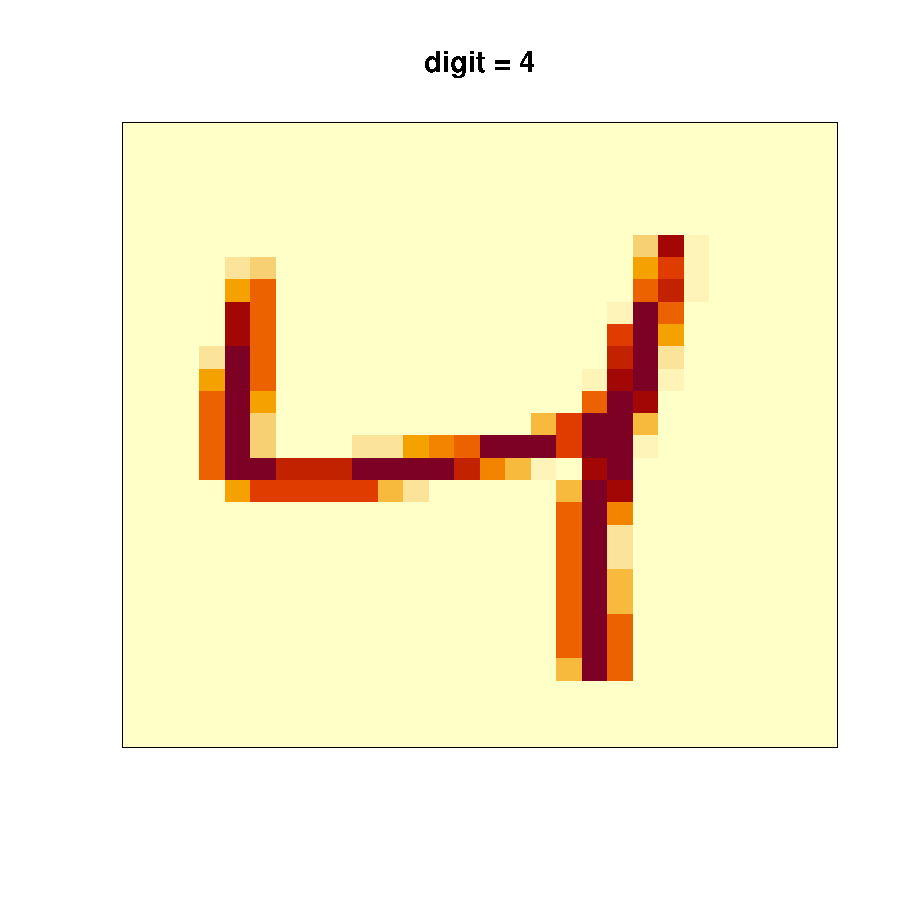
\includegraphics[width=\maxwidth]{figure/unnamed-chunk-33-1} 
\end{knitrout}

\subsection{2.2}
\begin{knitrout}
\definecolor{shadecolor}{rgb}{0.969, 0.969, 0.969}\color{fgcolor}\begin{kframe}
\begin{alltt}
\hlstd{X} \hlkwb{<-} \hlstd{mnist_example[[}\hlstr{"4"}\hlstd{]][}\hlnum{12}\hlopt{:} \hlnum{15}\hlstd{,} \hlnum{12}\hlopt{:} \hlnum{15}\hlstd{]}
\hlstd{K} \hlkwb{<-} \hlkwd{matrix}\hlstd{(}\hlkwd{c}\hlstd{(}\hlopt{-}\hlnum{0.5}\hlstd{,} \hlopt{-}\hlnum{0.5}\hlstd{,} \hlopt{-}\hlnum{0.5}\hlstd{,} \hlnum{1}\hlstd{,} \hlnum{1}\hlstd{,} \hlnum{1}\hlstd{,} \hlopt{-}\hlnum{0.5}\hlstd{,} \hlopt{-}\hlnum{0.5}\hlstd{,} \hlopt{-}\hlnum{0.5}\hlstd{) ,} \hlkwc{nrow} \hlstd{=} \hlnum{3}\hlstd{,} \hlkwc{byrow} \hlstd{=} \hlnum{TRUE}\hlstd{)}
\hlstd{K}
\end{alltt}
\begin{verbatim}
     [,1] [,2] [,3]
[1,] -0.5 -0.5 -0.5
[2,]  1.0  1.0  1.0
[3,] -0.5 -0.5 -0.5
\end{verbatim}
\begin{alltt}
\hlstd{X}
\end{alltt}
\begin{verbatim}
     [,1] [,2] [,3] [,4]
[1,]   56  250  116    0
[2,]    0  240  144    0
[3,]    0  198  150    0
[4,]    0  143  241    0
\end{verbatim}
\begin{alltt}
\hlstd{kernel_func} \hlkwb{<-} \hlkwa{function}\hlstd{(}\hlkwc{X_block}\hlstd{,} \hlkwc{K}\hlstd{)\{}
  \hlstd{res} \hlkwb{<-} \hlkwd{sum}\hlstd{(X_block}\hlopt{*}\hlstd{K)}
  \hlkwd{return}\hlstd{(res)}
\hlstd{\}}

\hlstd{convolution} \hlkwb{<-} \hlkwa{function}\hlstd{(}\hlkwc{X}\hlstd{,} \hlkwc{K}\hlstd{) \{}
  \hlstd{k_dim} \hlkwb{<-} \hlkwd{nrow}\hlstd{(K)}
  \hlstd{n_xrows} \hlkwb{<-} \hlkwd{nrow}\hlstd{(X)}
  \hlstd{n_xcols} \hlkwb{<-} \hlkwd{ncol}\hlstd{(X)}
  \hlstd{steps_down} \hlkwb{<-} \hlstd{n_xrows} \hlopt{-} \hlstd{k_dim} \hlopt{+} \hlnum{1}
  \hlstd{steps_right} \hlkwb{<-} \hlstd{n_xcols} \hlopt{-} \hlstd{k_dim} \hlopt{+} \hlnum{1}

  \hlstd{result} \hlkwb{<-} \hlkwd{matrix}\hlstd{(}\hlnum{0}\hlstd{,} \hlkwc{nrow} \hlstd{= steps_down,} \hlkwc{ncol} \hlstd{= steps_right)}

  \hlkwa{for} \hlstd{(i} \hlkwa{in} \hlnum{1}\hlopt{:}\hlstd{steps_down) \{}
       \hlstd{row_subset} \hlkwb{<-} \hlstd{i}\hlopt{:}\hlstd{(i} \hlopt{+} \hlstd{k_dim} \hlopt{-} \hlnum{1}\hlstd{)}
    \hlkwa{for} \hlstd{(j} \hlkwa{in} \hlnum{1}\hlopt{:}\hlstd{steps_right) \{}
      \hlstd{col_subset} \hlkwb{<-} \hlstd{j}\hlopt{:}\hlstd{(j} \hlopt{+} \hlstd{k_dim} \hlopt{-} \hlnum{1}\hlstd{)}
      \hlstd{X_block} \hlkwb{<-} \hlstd{X[row_subset, col_subset]}
      \hlstd{result[i, j]} \hlkwb{<-} \hlkwd{kernel_func}\hlstd{(X_block, K)}
    \hlstd{\}}
  \hlstd{\}}

  \hlkwd{return}\hlstd{(result)}
\hlstd{\}}

\hlkwd{convolution}\hlstd{(X,K)}
\end{alltt}
\begin{verbatim}
     [,1] [,2]
[1,]   -1   27
[2,]  -36  -36
\end{verbatim}
\end{kframe}
\end{knitrout}

\subsection{2.3}
Applying to function to the MNIST example 4 digit yields:

\begin{knitrout}
\definecolor{shadecolor}{rgb}{0.969, 0.969, 0.969}\color{fgcolor}\begin{kframe}
\begin{alltt}
\hlstd{conv_res} \hlkwb{<-} \hlkwd{convolution}\hlstd{(mnist_example[[}\hlstr{"4"}\hlstd{]], K)}
\hlkwd{image_func}\hlstd{(conv_res)}
\end{alltt}
\end{kframe}\begin{figure}
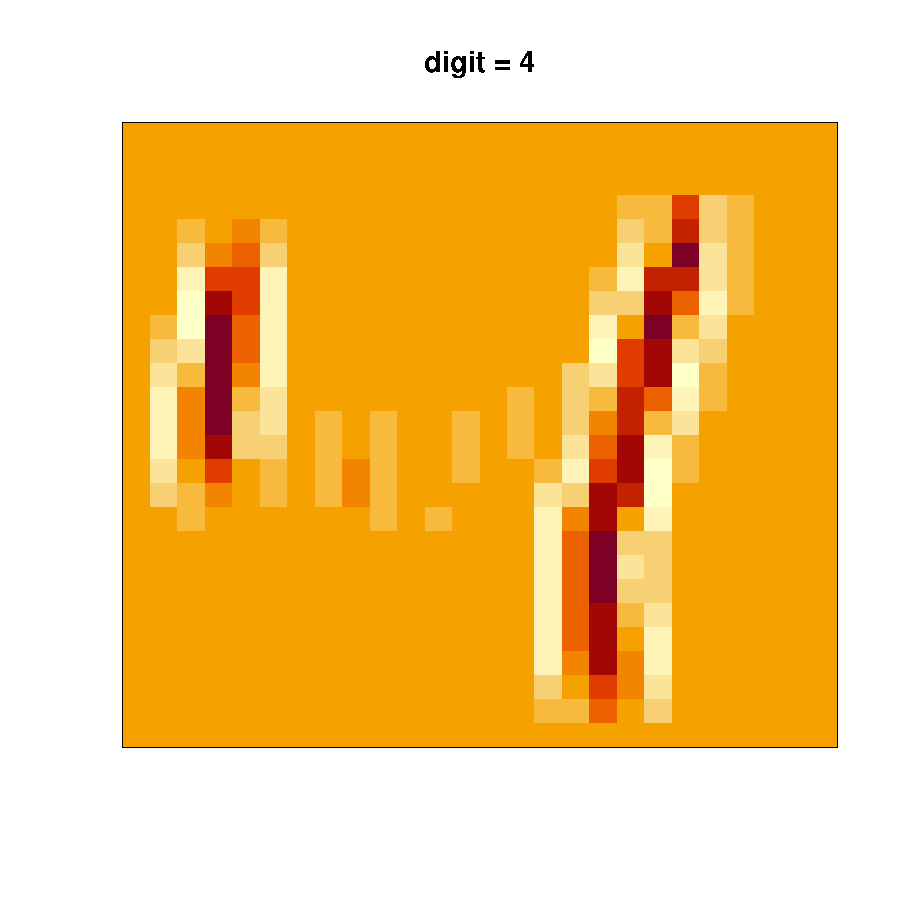
\includegraphics[width=\maxwidth]{figure/unnamed-chunk-35-1} \caption[Results from convulution function on mnist example]{Results from convulution function on mnist example}\label{fig:unnamed-chunk-35}
\end{figure}

\end{knitrout}

\subsection{2.4}
Now we add more functionality for bias as well as an activation function
\begin{knitrout}
\definecolor{shadecolor}{rgb}{0.969, 0.969, 0.969}\color{fgcolor}\begin{kframe}
\begin{alltt}
\hlstd{relu} \hlkwb{<-} \hlkwa{function}\hlstd{(}\hlkwc{x}\hlstd{)} \hlkwd{max}\hlstd{(}\hlnum{0}\hlstd{, x)}

\hlstd{convolutional_layer} \hlkwb{<-} \hlkwa{function}\hlstd{(}\hlkwc{X}\hlstd{,} \hlkwc{K}\hlstd{,} \hlkwc{b}\hlstd{,} \hlkwc{activation}\hlstd{)\{}
  \hlstd{conv_result} \hlkwb{<-} \hlkwd{convolution}\hlstd{(X,K)}
  \hlstd{conv_bias} \hlkwb{<-} \hlstd{conv_result} \hlopt{+} \hlstd{b}

  \hlstd{output} \hlkwb{<-}\hlkwd{apply}\hlstd{(conv_bias,} \hlkwc{MARGIN} \hlstd{=} \hlkwd{c}\hlstd{(}\hlnum{1}\hlstd{,} \hlnum{2}\hlstd{),} \hlkwc{FUN} \hlstd{= activation)}


  \hlkwd{return}\hlstd{(output)}

  \hlstd{\}}
\hlkwd{convolutional_layer}\hlstd{(X, K,} \hlnum{100}\hlstd{, relu)}
\end{alltt}
\begin{verbatim}
     [,1] [,2]
[1,]   99  127
[2,]   64   64
\end{verbatim}
\end{kframe}
\end{knitrout}

\subsection{2.5}
Now we apply the function on digit 4 and visualize the result.
\begin{knitrout}
\definecolor{shadecolor}{rgb}{0.969, 0.969, 0.969}\color{fgcolor}\begin{kframe}
\begin{alltt}
\hlstd{conv_layer_res} \hlkwb{<-} \hlkwd{convolutional_layer}\hlstd{(}\hlkwc{X}\hlstd{= mnist_example[[}\hlstr{"4"}\hlstd{]], K,} \hlkwc{b}\hlstd{=} \hlopt{-}\hlnum{150}\hlstd{, relu)}
\end{alltt}
\end{kframe}
\end{knitrout}

\begin{knitrout}
\definecolor{shadecolor}{rgb}{0.969, 0.969, 0.969}\color{fgcolor}\begin{kframe}
\begin{alltt}
\hlkwd{image_func}\hlstd{(conv_layer_res)}
\end{alltt}
\end{kframe}\begin{figure}
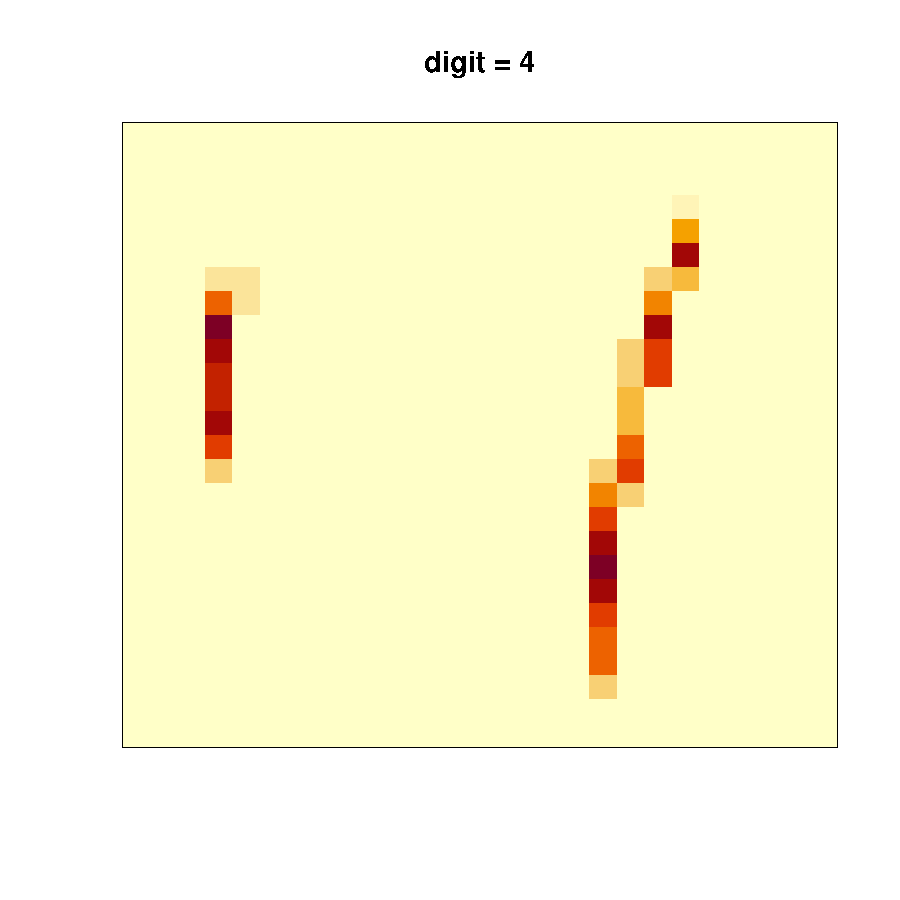
\includegraphics[width=\maxwidth]{figure/unnamed-chunk-38-1} \caption[Visualization of the convolutional layer result]{Visualization of the convolutional layer result}\label{fig:unnamed-chunk-38}
\end{figure}

\end{knitrout}

This seems to visualize the vertical lines in the digit 4.
\subsection{2.6}
Next we tranpose the filter and run the convolutional layer yet again with bias = -150

\begin{knitrout}
\definecolor{shadecolor}{rgb}{0.969, 0.969, 0.969}\color{fgcolor}\begin{kframe}
\begin{alltt}
\hlstd{conv_layer_res_t} \hlkwb{<-} \hlkwd{convolutional_layer}\hlstd{(}\hlkwc{X}\hlstd{= mnist_example[[}\hlstr{"4"}\hlstd{]],}
                                        \hlkwd{t}\hlstd{(K),} \hlkwc{b}\hlstd{=} \hlopt{-}\hlnum{150}\hlstd{, relu)}
\end{alltt}
\end{kframe}
\end{knitrout}

\begin{knitrout}
\definecolor{shadecolor}{rgb}{0.969, 0.969, 0.969}\color{fgcolor}\begin{kframe}
\begin{alltt}
\hlkwd{image_func}\hlstd{(conv_layer_res_t)}
\end{alltt}
\end{kframe}\begin{figure}
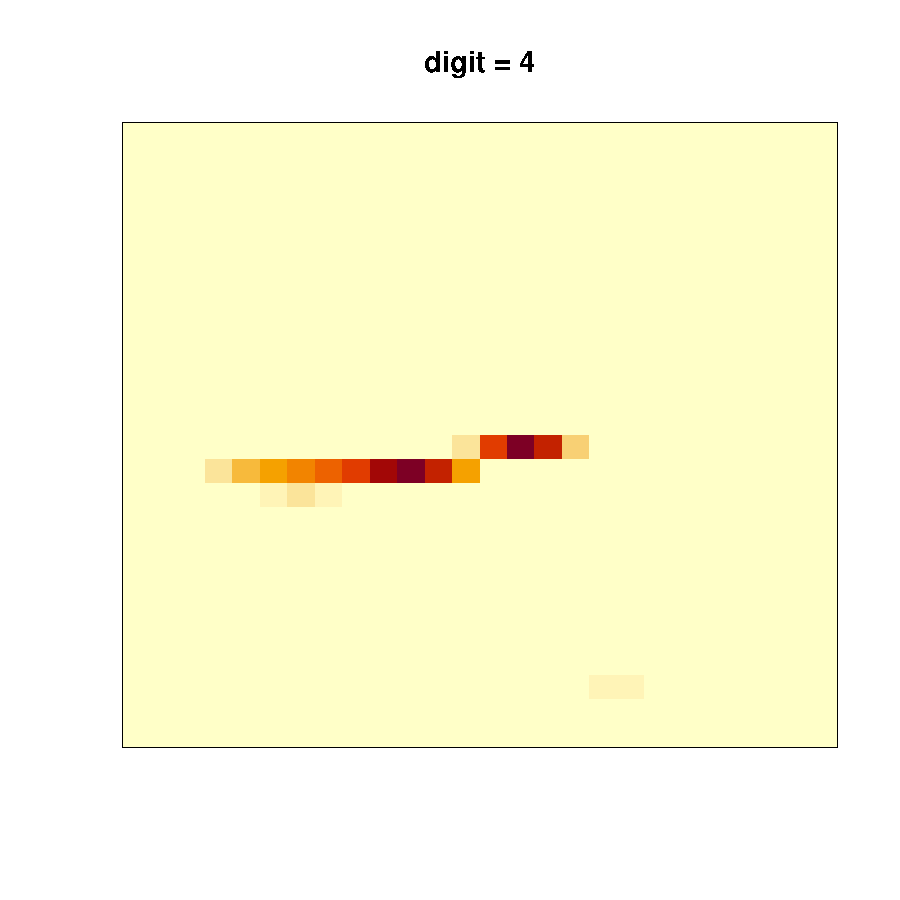
\includegraphics[width=\maxwidth]{figure/unnamed-chunk-40-1} \caption[Visualization of convolutional layer results with tranposed kernel ]{Visualization of convolutional layer results with tranposed kernel }\label{fig:unnamed-chunk-40}
\end{figure}

\end{knitrout}

Looking at the image, this transposed filter seems to illustrate the horizontal line in the digit 4. 
\subsection{2.7}
Now we implement a two by two, two stride max-pooling layer.
\begin{knitrout}
\definecolor{shadecolor}{rgb}{0.969, 0.969, 0.969}\color{fgcolor}\begin{kframe}
\begin{alltt}
\hlstd{X} \hlkwb{<-} \hlstd{mnist_example[[}\hlstr{"4"}\hlstd{]][}\hlnum{12}\hlopt{:} \hlnum{15}\hlstd{,} \hlnum{12}\hlopt{:} \hlnum{15}\hlstd{]}
\hlstd{X}
\end{alltt}
\begin{verbatim}
     [,1] [,2] [,3] [,4]
[1,]   56  250  116    0
[2,]    0  240  144    0
[3,]    0  198  150    0
[4,]    0  143  241    0
\end{verbatim}
\begin{alltt}
\hlstd{maxpool_layer} \hlkwb{<-} \hlkwa{function}\hlstd{(}\hlkwc{X}\hlstd{,} \hlkwc{size}\hlstd{=}\hlnum{2}\hlstd{)\{}
  \hlstd{n_xcols} \hlkwb{<-} \hlkwd{ncol}\hlstd{(X)}
  \hlstd{n_xrows} \hlkwb{<-} \hlkwd{nrow}\hlstd{(X)}

  \hlstd{steps_down} \hlkwb{<-} \hlstd{n_xrows} \hlopt \hlstd{size}
  \hlstd{steps_right} \hlkwb{<-} \hlstd{n_xcols}  \hlopt \hlstd{size}

  \hlcom{#indeces where to start each row and col subset}
  \hlstd{row_start} \hlkwb{<-} \hlkwd{seq}\hlstd{(}\hlkwc{from}\hlstd{=}\hlnum{1}\hlstd{,} \hlkwc{to}\hlstd{=n_xrows,} \hlkwc{by}\hlstd{=size)}
  \hlstd{col_start} \hlkwb{<-} \hlkwd{seq}\hlstd{(}\hlkwc{from}\hlstd{=}\hlnum{1}\hlstd{,} \hlkwc{to}\hlstd{=n_xcols,} \hlkwc{by}\hlstd{=size)}

    \hlstd{results} \hlkwb{<-} \hlkwd{matrix}\hlstd{(}\hlnum{NA}\hlstd{,} \hlkwc{nrow}\hlstd{=steps_down,} \hlkwc{ncol}\hlstd{=steps_right)}
    \hlkwa{for}\hlstd{(i} \hlkwa{in} \hlnum{1}\hlopt{:}\hlstd{steps_down)\{}

      \hlstd{r_subset} \hlkwb{<-} \hlstd{row_start[i]}\hlopt{:}\hlstd{(row_start[i]}\hlopt{+}\hlstd{size}\hlopt{-}\hlnum{1}\hlstd{)}

    \hlkwa{for}\hlstd{(j} \hlkwa{in} \hlnum{1}\hlopt{:}\hlstd{steps_right)\{}
      \hlstd{c_subset} \hlkwb{<-} \hlstd{col_start[j]}\hlopt{:}\hlstd{(col_start[j]}\hlopt{+}\hlstd{size}\hlopt{-}\hlnum{1}\hlstd{)}
      \hlstd{results[i,j]} \hlkwb{<-} \hlkwd{max}\hlstd{(X[r_subset, c_subset])}
      \hlstd{\}}
    \hlstd{\}}
  \hlkwd{return}\hlstd{(results)}
\hlstd{\}}

\hlkwd{maxpool_layer}\hlstd{(X)}
\end{alltt}
\begin{verbatim}
     [,1] [,2]
[1,]  250  144
[2,]  198  241
\end{verbatim}
\end{kframe}
\end{knitrout}

 \subsection{2.8}
 Now to put it all together and visualize the final output. 


\begin{knitrout}
\definecolor{shadecolor}{rgb}{0.969, 0.969, 0.969}\color{fgcolor}\begin{kframe}
\begin{alltt}
\hlstd{X} \hlkwb{<-} \hlstd{mnist_example[[}\hlstr{"4"}\hlstd{]]}

\hlstd{relu} \hlkwb{<-} \hlkwa{function}\hlstd{(}\hlkwc{x}\hlstd{)} \hlkwd{max}\hlstd{(}\hlnum{0}\hlstd{, x)}
\hlstd{output} \hlkwb{<-} \hlkwd{maxpool_layer}\hlstd{(}\hlkwd{convolutional_layer}\hlstd{(X, K,} \hlkwc{b}\hlstd{=}\hlopt{-}\hlnum{320}\hlstd{, relu))}
\end{alltt}
\end{kframe}
\end{knitrout}

\begin{knitrout}
\definecolor{shadecolor}{rgb}{0.969, 0.969, 0.969}\color{fgcolor}\begin{kframe}
\begin{alltt}
\hlkwd{image_func}\hlstd{(output)}
\end{alltt}
\end{kframe}\begin{figure}
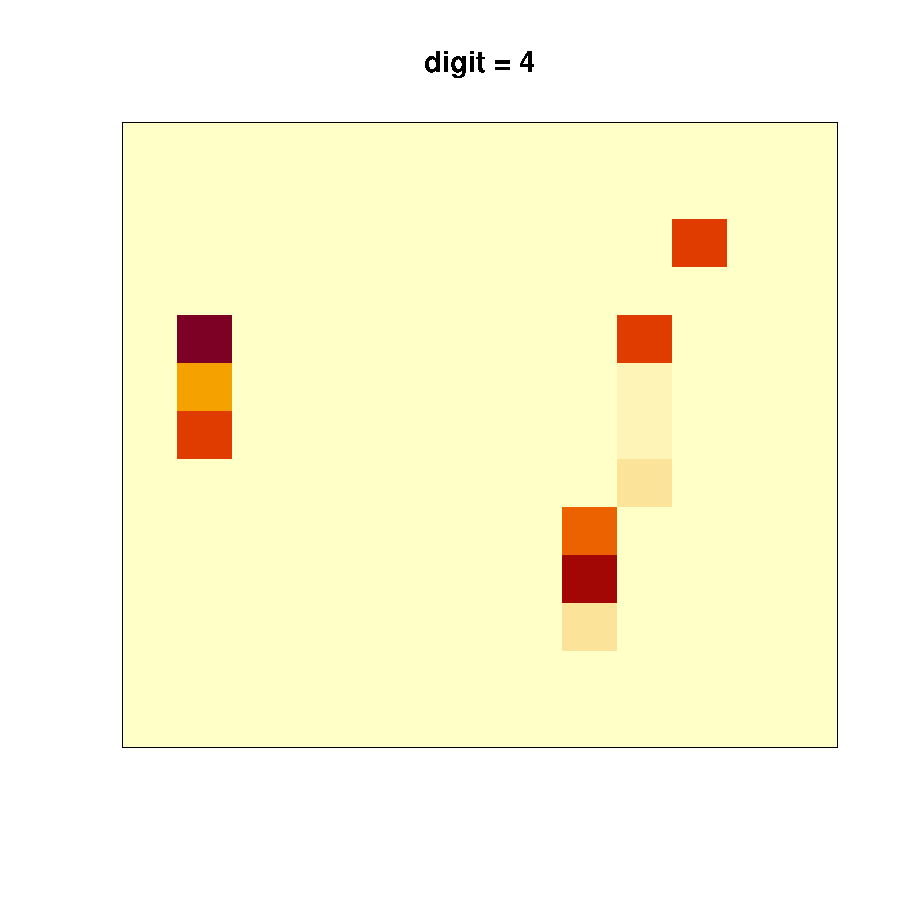
\includegraphics[width=\maxwidth]{figure/unnamed-chunk-43-1} \caption[Visualization of final result]{Visualization of final result}\label{fig:unnamed-chunk-43}
\end{figure}

\end{knitrout}

Looking at the results, then it seems like this is capturing the rough outlines of the vertical bars in the digit 4. 
\end{document}
